\documentclass[11pt,a4paper]{article}

\usepackage[provide=*,spanish]{babel}
\usepackage[utf8]{inputenc}
\usepackage[T1]{fontenc}
\usepackage{lmodern}
\usepackage[margin=2.35cm]{geometry}
\usepackage{amsmath}
\usepackage{booktabs}
\usepackage{longtable}
\usepackage{tabularx}
\usepackage{array}
\usepackage{enumitem}
\usepackage{listings}
\usepackage{xcolor}
\usepackage{microtype}
\usepackage{parskip}
\usepackage{titlesec}
\usepackage{hyperref}
\usepackage{graphicx}
\usepackage{caption}
\usepackage{subcaption}
\usepackage{float}

\definecolor{azulWCD}{RGB}{17,67,112}
\definecolor{azulClaro}{RGB}{232,241,249}
\definecolor{grisCodigo}{RGB}{247,247,247}
\definecolor{verdeCodigo}{RGB}{25,110,55}
\definecolor{rojoCodigo}{RGB}{145,35,35}
\definecolor{tituloColor}{RGB}{0,55,110}
\definecolor{reglaColor}{RGB}{0,90,160}

\hypersetup{
  colorlinks=true,
  linkcolor=azulWCD,
  urlcolor=azulWCD,
  citecolor=azulWCD,
  pdftitle={Balance de captura, reflexion y transmision, y letargia de neutrones en el WCD en funcion de la energia de inyeccion},
  pdfauthor={Jaime A. Betancourt}
}

\lstdefinestyle{pystyle}{
  language=Python,
  backgroundcolor=\color{grisCodigo},
  basicstyle=\ttfamily\footnotesize,
  keywordstyle=\color{azulWCD}\bfseries,
  commentstyle=\color{verdeCodigo}\itshape,
  stringstyle=\color{rojoCodigo},
  breaklines=true,
  breakatwhitespace=false,
  frame=single,
  rulecolor=\color{gray!40},
  tabsize=2,
  showstringspaces=false,
  columns=fullflexible,
  keepspaces=true
}
\lstset{style=pystyle}

\titleformat{\section}{\normalfont\Large\bfseries\color{azulWCD}}
  {\thesection.}{0.6em}{}
\titleformat{\subsection}{\normalfont\large\bfseries}
  {\thesubsection.}{0.5em}{}
\setlist{itemsep=0.25em,topsep=0.4em}
\renewcommand{\arraystretch}{1.18}
\setlength{\emergencystretch}{2em}

\newcommand{\codigo}[1]{\nolinkurl{#1}}
\newcommand{\archivo}[1]{\path{#1}}
\newcommand{\var}[1]{\texttt{#1}}

\begin{document}
\pagestyle{empty}

%------------------------------------------------
% PORTADA
%------------------------------------------------

\begin{titlepage}
\begin{center}

\vspace*{0.5cm}
\textcolor{reglaColor}{\rule{\linewidth}{1.2pt}}

\vspace{1.3cm}
{\Large\scshape Universidad Industrial de Santander}\\[0.2cm]
{\large Escuela de Física --- Facultad de Ciencias}\\[0.2cm]
{\large Doctorado en Física}

\vspace{2.2cm}
{\Huge\bfseries\color{tituloColor} Balance de captura, reflexión y\\[0.2cm]
transmisión, y letargía de neutrones\\[0.2cm] en el WCD según la energía de inyección}

\vspace{1.8cm}
{\large\textbf{Informe técnico}}

\vspace{0.6cm}
\begin{minipage}{0.82\linewidth}
\centering
\textit{``Cómo cambia la respuesta del detector según la energía con la que llega el neutrón: de 1\,meV a 10\,keV, en agua pura y con NaCl''}
\end{minipage}

\vfill

{\large\textbf{Autor}}\\[0.15cm]
Jaime A. Betancourt\\[0.1cm]
Doctorado en Física, Universidad Industrial de Santander

\vspace{1.2cm}
\textcolor{reglaColor}{\rule{0.5\linewidth}{0.6pt}}

\vspace{1cm}
16 de septiembre de 2026

\vspace{1cm}
\textcolor{reglaColor}{\rule{\linewidth}{1.2pt}}

\end{center}
\end{titlepage}

\pagestyle{plain}

\begin{abstract}
Este informe documenta e interpreta, para un lector con acceso al repositorio de la tesis pero sin conocimiento previo del análisis, el balance de captura/reflexión/transmisión y la letargía logarítmica $\xi$ de neutrones simulados (Geant4/MEIGA) en el detector Cherenkov de agua (WCD) con agua pura y con soluciones de NaCl (2.5\,\%, 5\,\%, 10\,\% en masa), \textbf{en función de la energía de inyección}: 1\,meV, 10\,meV, 25\,meV, 100\,meV y 10\,keV (cinco corridas de 100\,000 neutrones cada una, cuatro concentraciones cada una --20 corridas en total). Estas corridas pertenecen a la \textbf{primera de dos campañas de simulación} de la tesis, sin el tratamiento térmico $S(\alpha,\beta)$ para el hidrógeno ligado en moléculas de agua (sección~\ref{sec:campanas}). A diferencia de un informe anterior sobre este mismo tema, aquí el análisis parte de un único archivo de
seguimiento paso a paso del neutrón primario (\codigo{interaccion-completa-neutrones.txt}) que \textbf{no incluye el material} en el que ocurre cada interacción, así que la clasificación captura/reflexión/transmisión se hace por geometría (posición final del neutrón) en vez de por material; esta limitación, y sus implicaciones, se explican en la
sección~\ref{sec:variables}. El resultado central es un \textbf{cruce de signo} en la letargía media de la historia completa de un neutrón capturado, $\langle\xi\rangle$, que pasa de negativa (por debajo del equilibrio térmico del agua, $\sim$1--25\,meV) a positiva (por encima de él, $\sim$100\,meV--10\,keV) justo alrededor de la temperatura ambiente del moderador, y una fracción de captura que \emph{no} es monótona con la energía en presencia de NaCl (máximo en 100\,meV).
\end{abstract}

\tableofcontents

\section{Objeto y alcance del informe}

El detector Cherenkov de agua (\textit{Water Cherenkov Detector}, WCD) que se modela en esta tesis responde, en última instancia, a neutrones que se moderan y se capturan  dentro de su volumen sensible. La caracterización de \emph{cómo} se comporta un neutrón dentro del tanque --cuántos se capturan, cuántos rebotan, cuántos lo atraviesan, y cómo cambia su energía en el camino-- ya se documentó, para una única energía de inyección (25\,meV, neutrones ya termalizados, con el tratamiento térmico $S(\alpha,\beta)$ activado --ver sección~\ref{sec:campanas}) y usando un pipeline con información de material, en una versión anterior de este informe.

Este informe reemplaza ese análisis por uno más amplio: la misma caracterización, pero repetida en \textbf{cinco energías de inyección distintas} (1\,meV, 10\,meV, 25\,meV, 100\,meV y 10\,keV), para ver cómo cambia la respuesta del detector según la energía con la que el neutrón llega al tanque -- algo relevante porque un WCD de campo real no recibe neutrones monoenergéticos, sino un espectro que depende de la humedad del suelo y de la moderación atmosférica previa. A cambio de cubrir cinco energías en vez de una, este análisis parte de una fuente de datos más simple (un solo archivo por corrida, sin información de material) que impone una limitación importante, explicada en detalle en
la sección~\ref{sec:variables}: no es posible distinguir captura ``en el medio activo'' de captura ``en la estructura'' como sí se podía en el informe anterior. Además, como se explica en la sección~\ref{sec:campanas}, esta campaña de cinco energías \textbf{no incluye} el tratamiento térmico $S(\alpha,\beta)$ que sí tenía la corrida del informe anterior, así que las cifras de captura de ambos informes tampoco son directamente comparables por esa segunda razón.

\section{Dos campañas de simulación: con y sin tratamiento térmico S($\alpha,\beta$)}
\label{sec:campanas}

Antes de leer los resultados, es importante que quien consulte este repositorio tenga clara la procedencia de los datos: las cifras de este informe provienen de una \textbf{campaña de simulación} concreta, y existe una \textbf{segunda campaña}, con una configuración física distinta, cuyos primeros resultados --en particular la fracción de captura-- ya se observan distintos de los de aquí. Ambas campañas comparten el mismo framework Geant4/MEIGA, la misma geometría del tanque y los mismos materiales de estructura, pero \textbf{no son directamente comparables cifra a cifra}:

\begin{itemize}
  \item \textbf{Campaña 1 (``primeras simulaciones''), la que documenta este informe.} Cinco energías de inyección (1\,meV, 10\,meV, 25\,meV, 100\,meV, 10\,keV) por cuatro concentraciones de NaCl (agua pura, 2.5\,\%, 5\,\%, 10\,\%) --20 corridas de 100\,000 neutrones--, clasificadas por geometría (sección~\ref{sec:pipeline}) porque el archivo de trazabilidad no registra el material de cada interacción. \textbf{Estas corridas no incluyen el tratamiento térmico $S(\alpha,\beta)$} para el hidrógeno ligado en moléculas de agua: el transporte de neutrones subtérmicos usa la sección eficaz libre estándar de Geant4/\codigo{QGSP\_BERT\_HP} para el hidrógeno, sin el modelo de red molecular que modula la dispersión elástica cerca y por debajo del equilibrio térmico del agua. \textbf{Esta es la campaña sobre la que se apoya el análisis completo de la tesis.}
  \item \textbf{Campaña 2 (exploratoria), con S($\alpha,\beta$).} Una única energía de inyección ejecutada hasta ahora --\textbf{25\,meV}, verificada directamente en \codigo{neutrones-incidentes.tsv} (\var{pre\_energy\_MeV} $=2.499996\times10^{-8}$\,MeV en las cuatro concentraciones)-- con clasificación por material (informe complementario \textit{Informe-tecnico-Estructura-Archivos-Simulacion} y los notebooks \codigo{analisis\_moderacion\_captura\_neutrones\_\_agua-*.ipynb}). \textbf{Estas corridas sí incluyen $S(\alpha,\beta)$.} En disco, esta campaña vive en la carpeta \codigo{25meV/}, correctamente nombrada. Se corrieron agua pura, 2.5\,\%, 5\,\% y 10\,\% de NaCl a esa energía; no existe todavía una versión de la Campaña 2 con las otras cuatro energías de la Campaña 1.
\end{itemize}

Como ambas campañas comparten el punto de 25\,meV --elegido en la Campaña 2 precisamente para poner a prueba el régimen térmico, alrededor de la energía térmica del medio, donde $S(\alpha,\beta)$ más debería importar-- \textbf{ese es el punto natural de comparación directa entre ellas}. La diferencia entre campañas no es cosmética: $S(\alpha,\beta)$ modifica la sección eficaz de dispersión elástica del hidrógeno ligado precisamente en ese rango de energías. \textbf{No debe darse por sentado que el balance de captura/reflexión/transmisión ni la letargía de una campaña reproducen los de la otra a 25\,meV} --de hecho, la fracción de captura ya se observa distinta entre ambas a esa misma energía. La comparación sistemática cifra a cifra entre campañas a 25\,meV, y la eventual extensión de la Campaña 2 a las otras cuatro energías, queda como trabajo pendiente (sección~\ref{sec:futuro}).

\section{Contexto: por qué se caracteriza así un detector de humedad de suelo}
\label{sec:contexto}

La técnica de \textbf{sensado de neutrones cósmico} (\textit{Cosmic-Ray Neutron Sensing}, CRNS) mide la humedad del suelo de forma no invasiva a partir de un hecho físico simple: el hidrógeno es, por mucho, el núcleo más eficiente para moderar (frenar) neutrones rápidos producidos por la radiación cósmica en la atmósfera. Cuanta más agua contiene el suelo bajo un detector, más se moderan y se absorben los neutrones que provienen del suelo, y por tanto \emph{menor} es el flujo de neutrones epitérmicos/rápidos que un detector situado sobre la superficie llega a contar. Un WCD --diseñado originalmente para detectar muones y electrones mediante luz Cherenkov-- puede, en principio,
adaptarse para actuar como uno de estos detectores de neutrones si su respuesta a la captura de neutrones térmicos dentro de su propio tanque de agua está bien caracterizada.

Un detector de campo real, sin embargo, no recibe un haz monoenergético: recibe una mezcla de neutrones que llegan con distintas energías según cuánto se moderaron en el suelo y en la atmósfera antes de llegar al detector. Por eso, además de caracterizar la respuesta a una energía fija (como hacía el informe anterior, a 25\,meV con $S(\alpha,\beta)$), interesa saber \textbf{cómo cambia esa respuesta con la energía de inyección}: si el balance de captura/reflexión/transmisión y la física de moderación ($\xi$, $N$) dependen fuertemente de la energía, entonces la forma del espectro de neutrones que llega al detector --no solo su intensidad total-- importa para interpretar la señal en términos de
humedad de suelo. Ese es el objetivo de este informe.

\section{Configuración de la simulación}
\label{sec:sim}

Cada una de las 20 corridas analizadas en este informe simula \textbf{100000 neutrones primarios}, inyectados verticalmente hacia abajo desde \textbf{70 cm} de altura sobre el tanque, con una energía inicial monoenergética que toma uno de cinco valores: \textbf{1 meV, 10 meV, 25 meV, 100 meV o 10 keV}. El tanque, la geometría y los materiales de estructura (acero inoxidable, Tyvek) son los mismos que en el resto de la tesis; el medio activo es agua pura o una solución de NaCl a 2.5 \%, 5 \% o 10 \% en masa, según la corrida. El transporte de neutrones usa Geant4 con física de alta precisión (\codigo{QGSP\_BERT\_HP}); a diferencia del resto de la tesis, \textbf{esta campaña de simulación (Campaña 1, sección~\ref{sec:campanas}) no incluye} el tratamiento térmico $S(\alpha,\beta)$ para el hidrógeno ligado en moléculas de agua.

\textbf{Nota sobre el nombre de una de las carpetas de datos}: la corrida etiquetada como ``10\,keV'' vive, en el disco, en una carpeta llamada \codigo{1keV/}. La energía de inyección real se verificó de manera independiente por dos vías distintas antes de usar estos datos: (1) la columna de energía cinética inicial de \codigo{interaccion-completa-neutrones.txt} vale $9.99997\times10^{-3}$\,MeV en las 100\,000 historias, y (2) el log crudo de Geant4 (\codigo{Flujo-100000N-1KeV-H2O-pura.txt}) imprime explícitamente, al generar cada partícula primaria, \var{Particle Kinetic Energy = 9.99997e-06 GeV} --el mismo valor, $\approx 10$\,keV, no 1\,keV. El nombre de la carpeta (y del archivo de flujo de entrada que Geant4 leyó, \codigo{100000N-1keV.txt}) es, con toda probabilidad, un error heredado de una etapa anterior de generación de esos archivos de flujo; este informe usa la energía verificada (10\,keV) en todo momento. (La carpeta \codigo{25meV/} de la Campaña 2, sección~\ref{sec:campanas}, sí está correctamente nombrada: 25\,meV, verificado por el mismo procedimiento.)

\section{Trazabilidad de los datos: de la simulación a las variables}
\label{sec:pipeline}

A diferencia del informe anterior (que combinaba cuatro archivos TSV con información de material), este análisis parte de un único archivo por corrida: \archivo{interaccion-completa-neutrones.txt}, con el registro paso a paso \emph{solo} del neutrón primario (\var{track\_id}=1, \var{parent\_id}=0) en 13 columnas: número de paso, partícula, \var{track\_id}, \var{parent\_id}, energía cinética inicial, posición inicial $(x_1,y_1,z_1)$, posición final $(x_2,y_2,z_2)$, energía cinética final, y el proceso físico del paso (\var{Transportation}, \var{hadElastic}, \var{nCapture}, \var{neutronInelastic}, y ocasionalmente \var{Decay}). \textbf{No hay columna de material.} Cuando este archivo no venía pre-generado para una corrida, se genera automáticamente filtrando el archivo crudo completo \archivo{informacion-completa.txt} (que sí incluye todas las partículas secundarias) por esas tres condiciones.

Cada historia de neutrón (\var{event\_id}) se identifica dentro del archivo por el reinicio del número de paso a 1. A partir de ahí se calculan, para cada corrida, el balance
(sección~\ref{sec:balance}), la letargía por régimen de energía (sección~\ref{sec:regimen}) y la letargía/$N$ de la historia completa de los neutrones capturados (secciones~\ref{sec:xi} y~\ref{sec:N}).

\section{Variables analizadas}
\label{sec:variables}

\subsection{Limitación central: sin columna de material}
\label{sec:limitacion}

Como \archivo{interaccion-completa-neutrones.txt} no distingue en qué material ocurre cada interacción, \textbf{no es posible reproducir aquí la distinción ``capturado en el medio activo'' vs.\ ``capturado en la estructura''} que sí se hacía en el informe anterior (con los cuatro TSV que sí incluían material). En este informe, ``Capturado'' significa simplemente que en algún paso de la historia del neutrón ocurrió \var{nCapture}, sin importar el material -- una definición más amplia que el $\eta_{\text{Cap}}$ del resto de la tesis, y por lo tanto \textbf{no directamente comparable} con esos números. De la misma manera, ``dentro del volumen detector'' (usado para el análisis por
régimen de energía, sección~\ref{sec:regimen}) se aproxima con la altura $z$ y las coordenadas $x$ e $y$ a la que el neutrón entra al tanque (detectada automáticamente de los datos, dentro de la geometría), no con el material.

\subsection{Coeficiente de captura, reflexión y transmisión}
\label{sec:balance}

Los 100000 neutrones inyectados de cada corrida se clasifican en seis categorías mutuamente excluyentes y exhaustivas:

\begin{itemize}
  \item \textbf{Capturado}: en algún paso de su historia ocurrió \var{nCapture} ( en el medio detector,  ver limitación arriba).
  \item \textbf{Reflejado}: no capturado; su última posición registrada sale por la misma cara de la caja del mundo de Geant4 por la que entró (arriba).
  \item \textbf{Transmitido}: no capturado; sale por la cara opuesta (abajo), habiendo atravesado  todo el volumen.
  \item \textbf{Escape lateral}: no capturado; sale por un costado de la caja del mundo 
  %-- categoría  que el balance de tres términos del resto de la tesis no tiene, necesaria aquí porque no hay información de material para decidir si ese neutrón realmente atravesó el tanque.
  \item \textbf{Inelástico terminal}: el último proceso registrado es \var{neutronInelastic} sin \var{nCapture} posterior.
  % -- el neutrón primario cambia de identidad sin que se etiquete como captura (mismo fenómeno documentado para el PMT de vidrio en otras partes de la tesis).
  %\item \textbf{Otro (proceso final atípico)}: residual, para historias que no encajan en ninguna de las anteriores (p.\ ej.\ un proceso \var{Decay} visto en 1 de cada 100\,000 historias en un par de corridas de baja energía) -- se reporta aparte en vez de forzarlas a otra categoría.
\end{itemize}

Los límites de la caja del mundo (para decidir reflejado/transmitido/escape lateral) se detectan automáticamente a partir de los propios datos en cada corrida (no están fijados de antemano), y salieron idénticos en las 20 corridas ($|x|,|y|<2750$ mm, $|z|<3000$ mm), confirmando que la geometría no cambia entre energías ni concentraciones. La figura~\ref{fig:balance} muestra este balance para las cinco energías, agrupado por medio.

\begin{figure}[H]
  \centering
  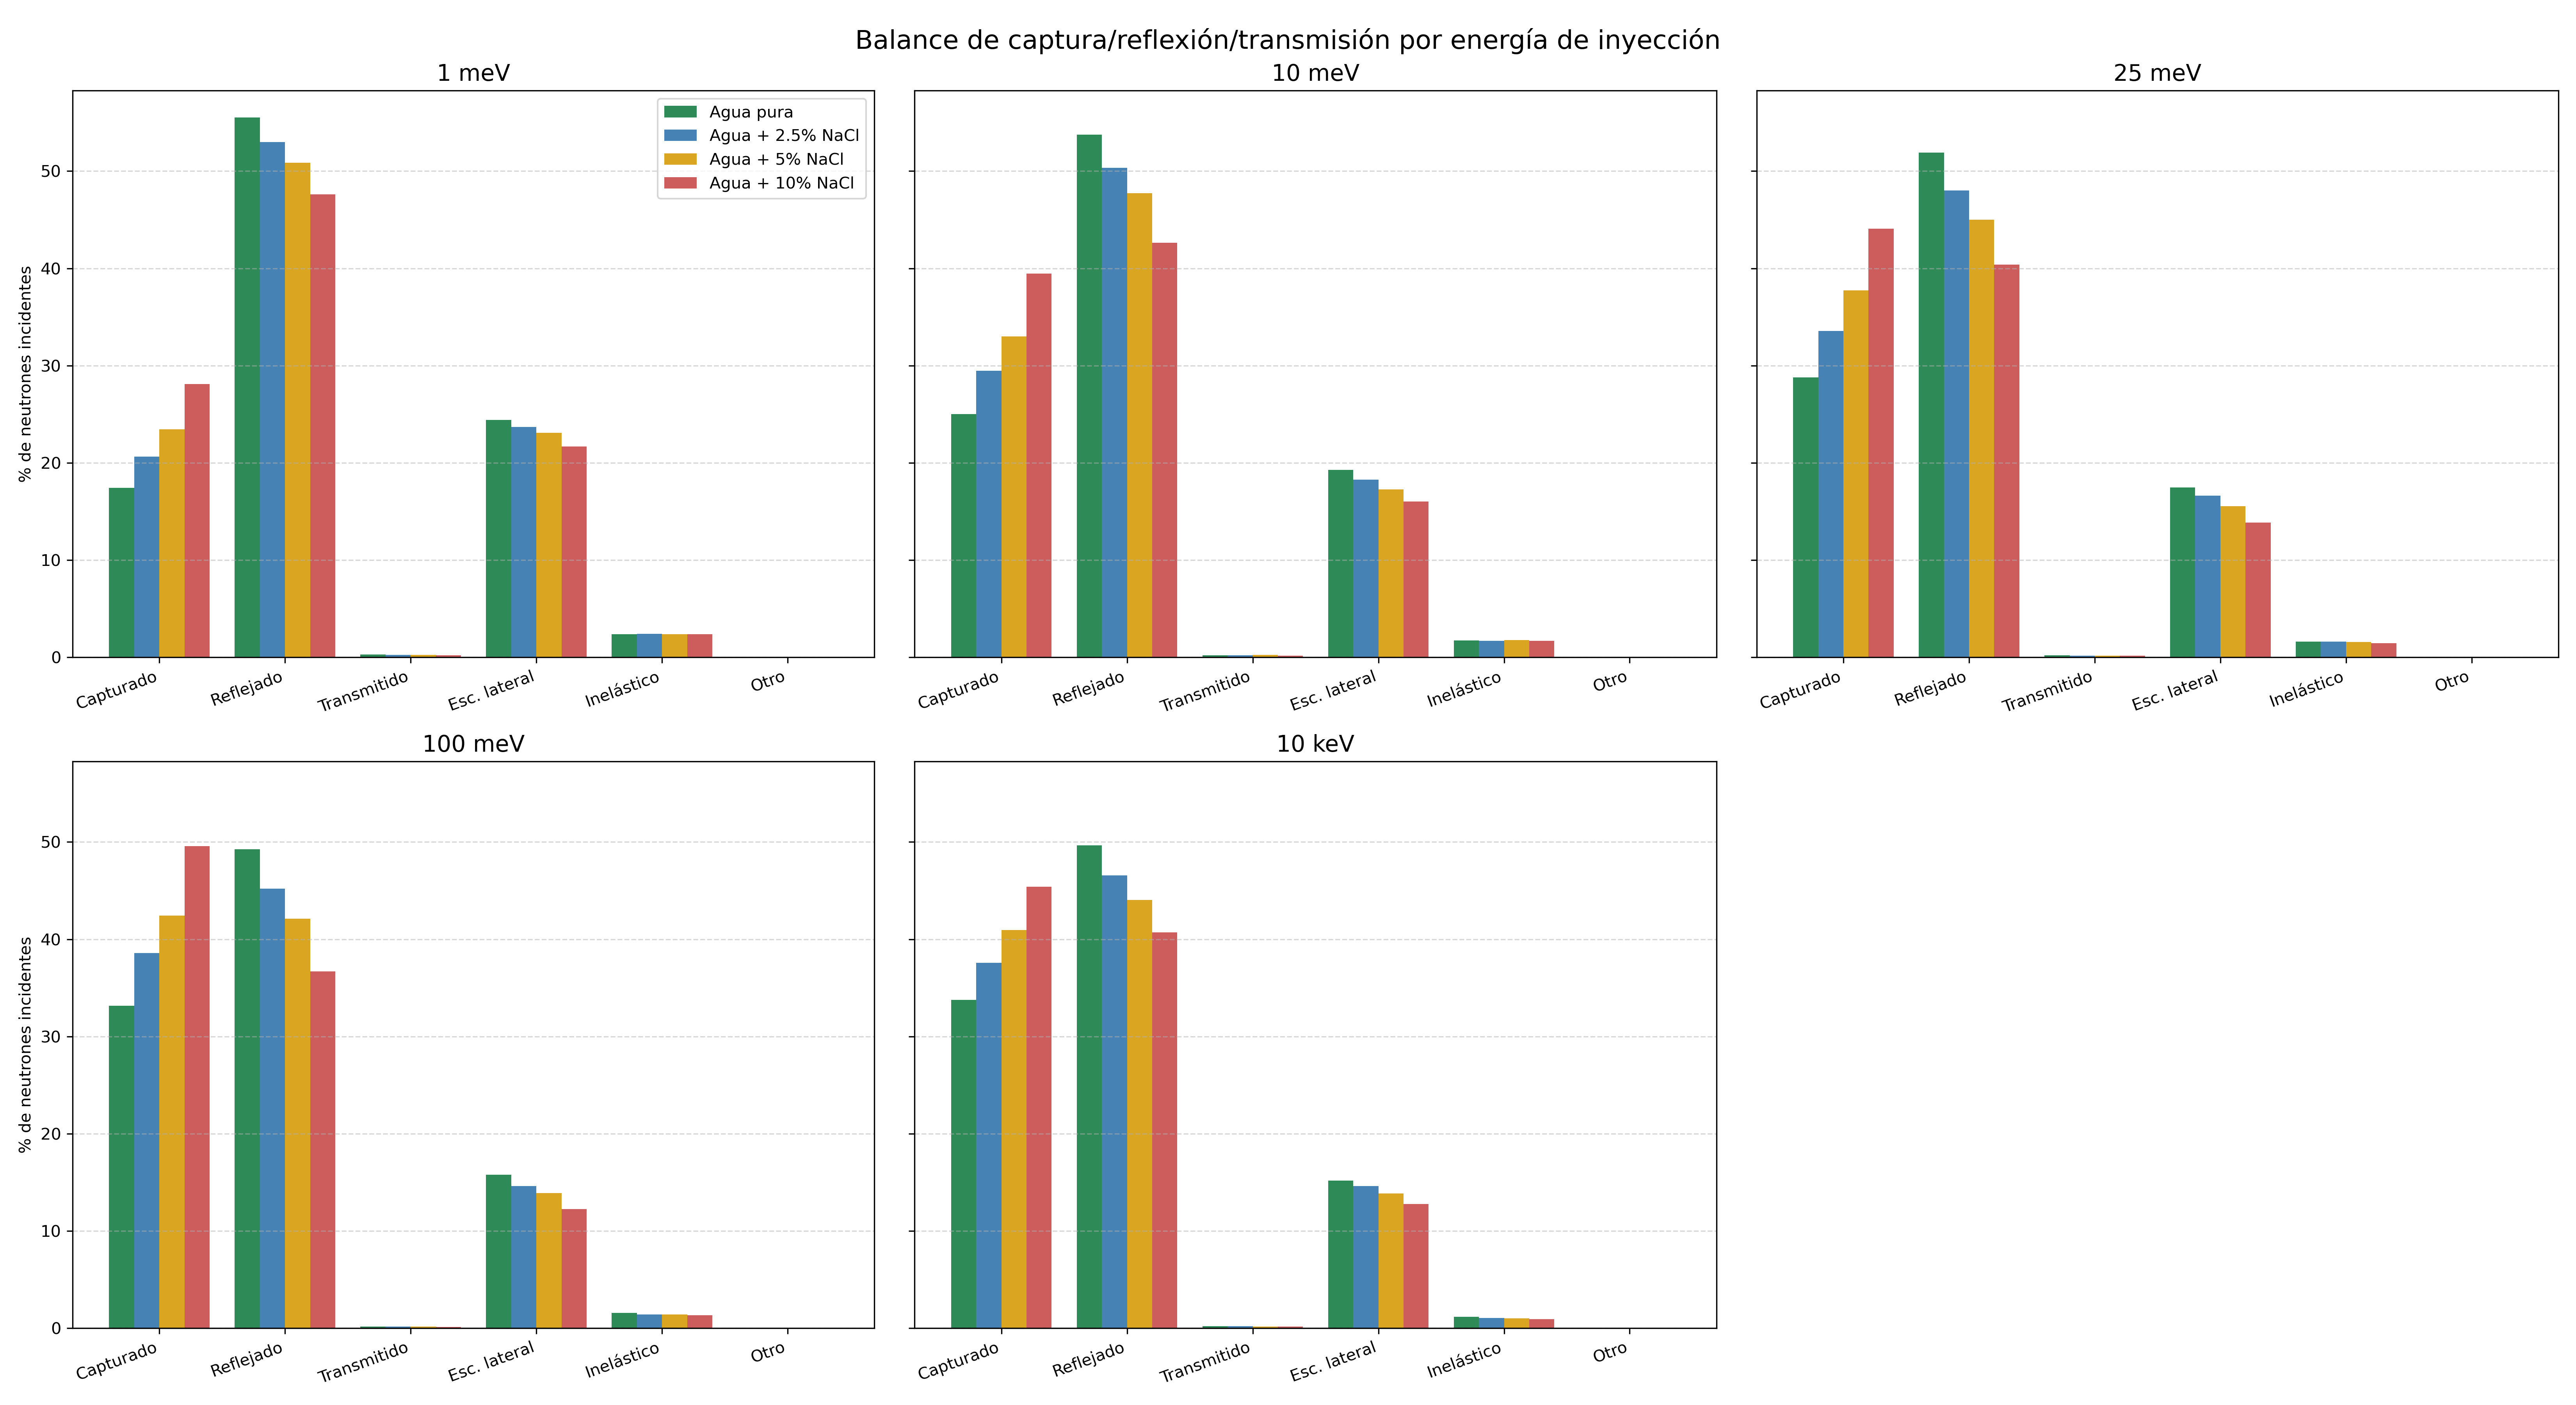
\includegraphics[width=\linewidth]{figuras-analisis-energia/balance_por_energia.png}
  \caption{Balance de los 100000 neutrones inyectados, por energía de inyección y medio. La captura sube con el NaCl en las cinco energías, pero no de forma monótona con la energía en presencia de NaCl (ver sección~\ref{sec:resultados}).}
  \label{fig:balance}
\end{figure}

\subsection{Letargía por régimen de energía}
\label{sec:regimen}

Restringido a los pasos dentro del volumen detector (aproximado por la altura $z$ de entrada al tanque, detectada automáticamente), cada paso se clasifica según su energía \emph{inicial} en uno de cuatro regímenes pedidos --frío (1--10meV), térmico (10--100meV), epitérmico (100meV--1eV) e intermedio (1eV--1keV). Dentro de cada régimen se calcula la letargía ganada por colisión, $\xi_{\text{régimen}} = \langle\ln(E_{\text{inicial}}/E_{\text{final}})\rangle$ promediada sobre las colisiones \var{hadElastic} de ese régimen -- el ``poder de moderación'' local del medio en esa banda de energía.

\textbf{El régimen Intermedio (1eV--1keV) depende de la energía de inyección}, no es siempre vacío ni siempre poblado: con fuente en o por debajo de 100meV nunca se alcanza esa banda (ni siquiera por una fluctuación térmica de \textit{up-scattering}, cuya probabilidad cae exponencialmente con la distancia en unidades de $kT\approx25$--$30$ meV); con fuente en 1keV, en cambio, el neutrón parte por encima de esa banda y la atraviesa como parte normal de su descenso de moderación. La figura~\ref{fig:hasta_donde} lo muestra directamente con los datos, comparando agua pura a 25meV (banda vacía) y a 1keV (banda poblada, con la energía máxima observada marcada).

\begin{figure}[H]
  \centering
  \begin{subfigure}[b]{0.49\linewidth}
    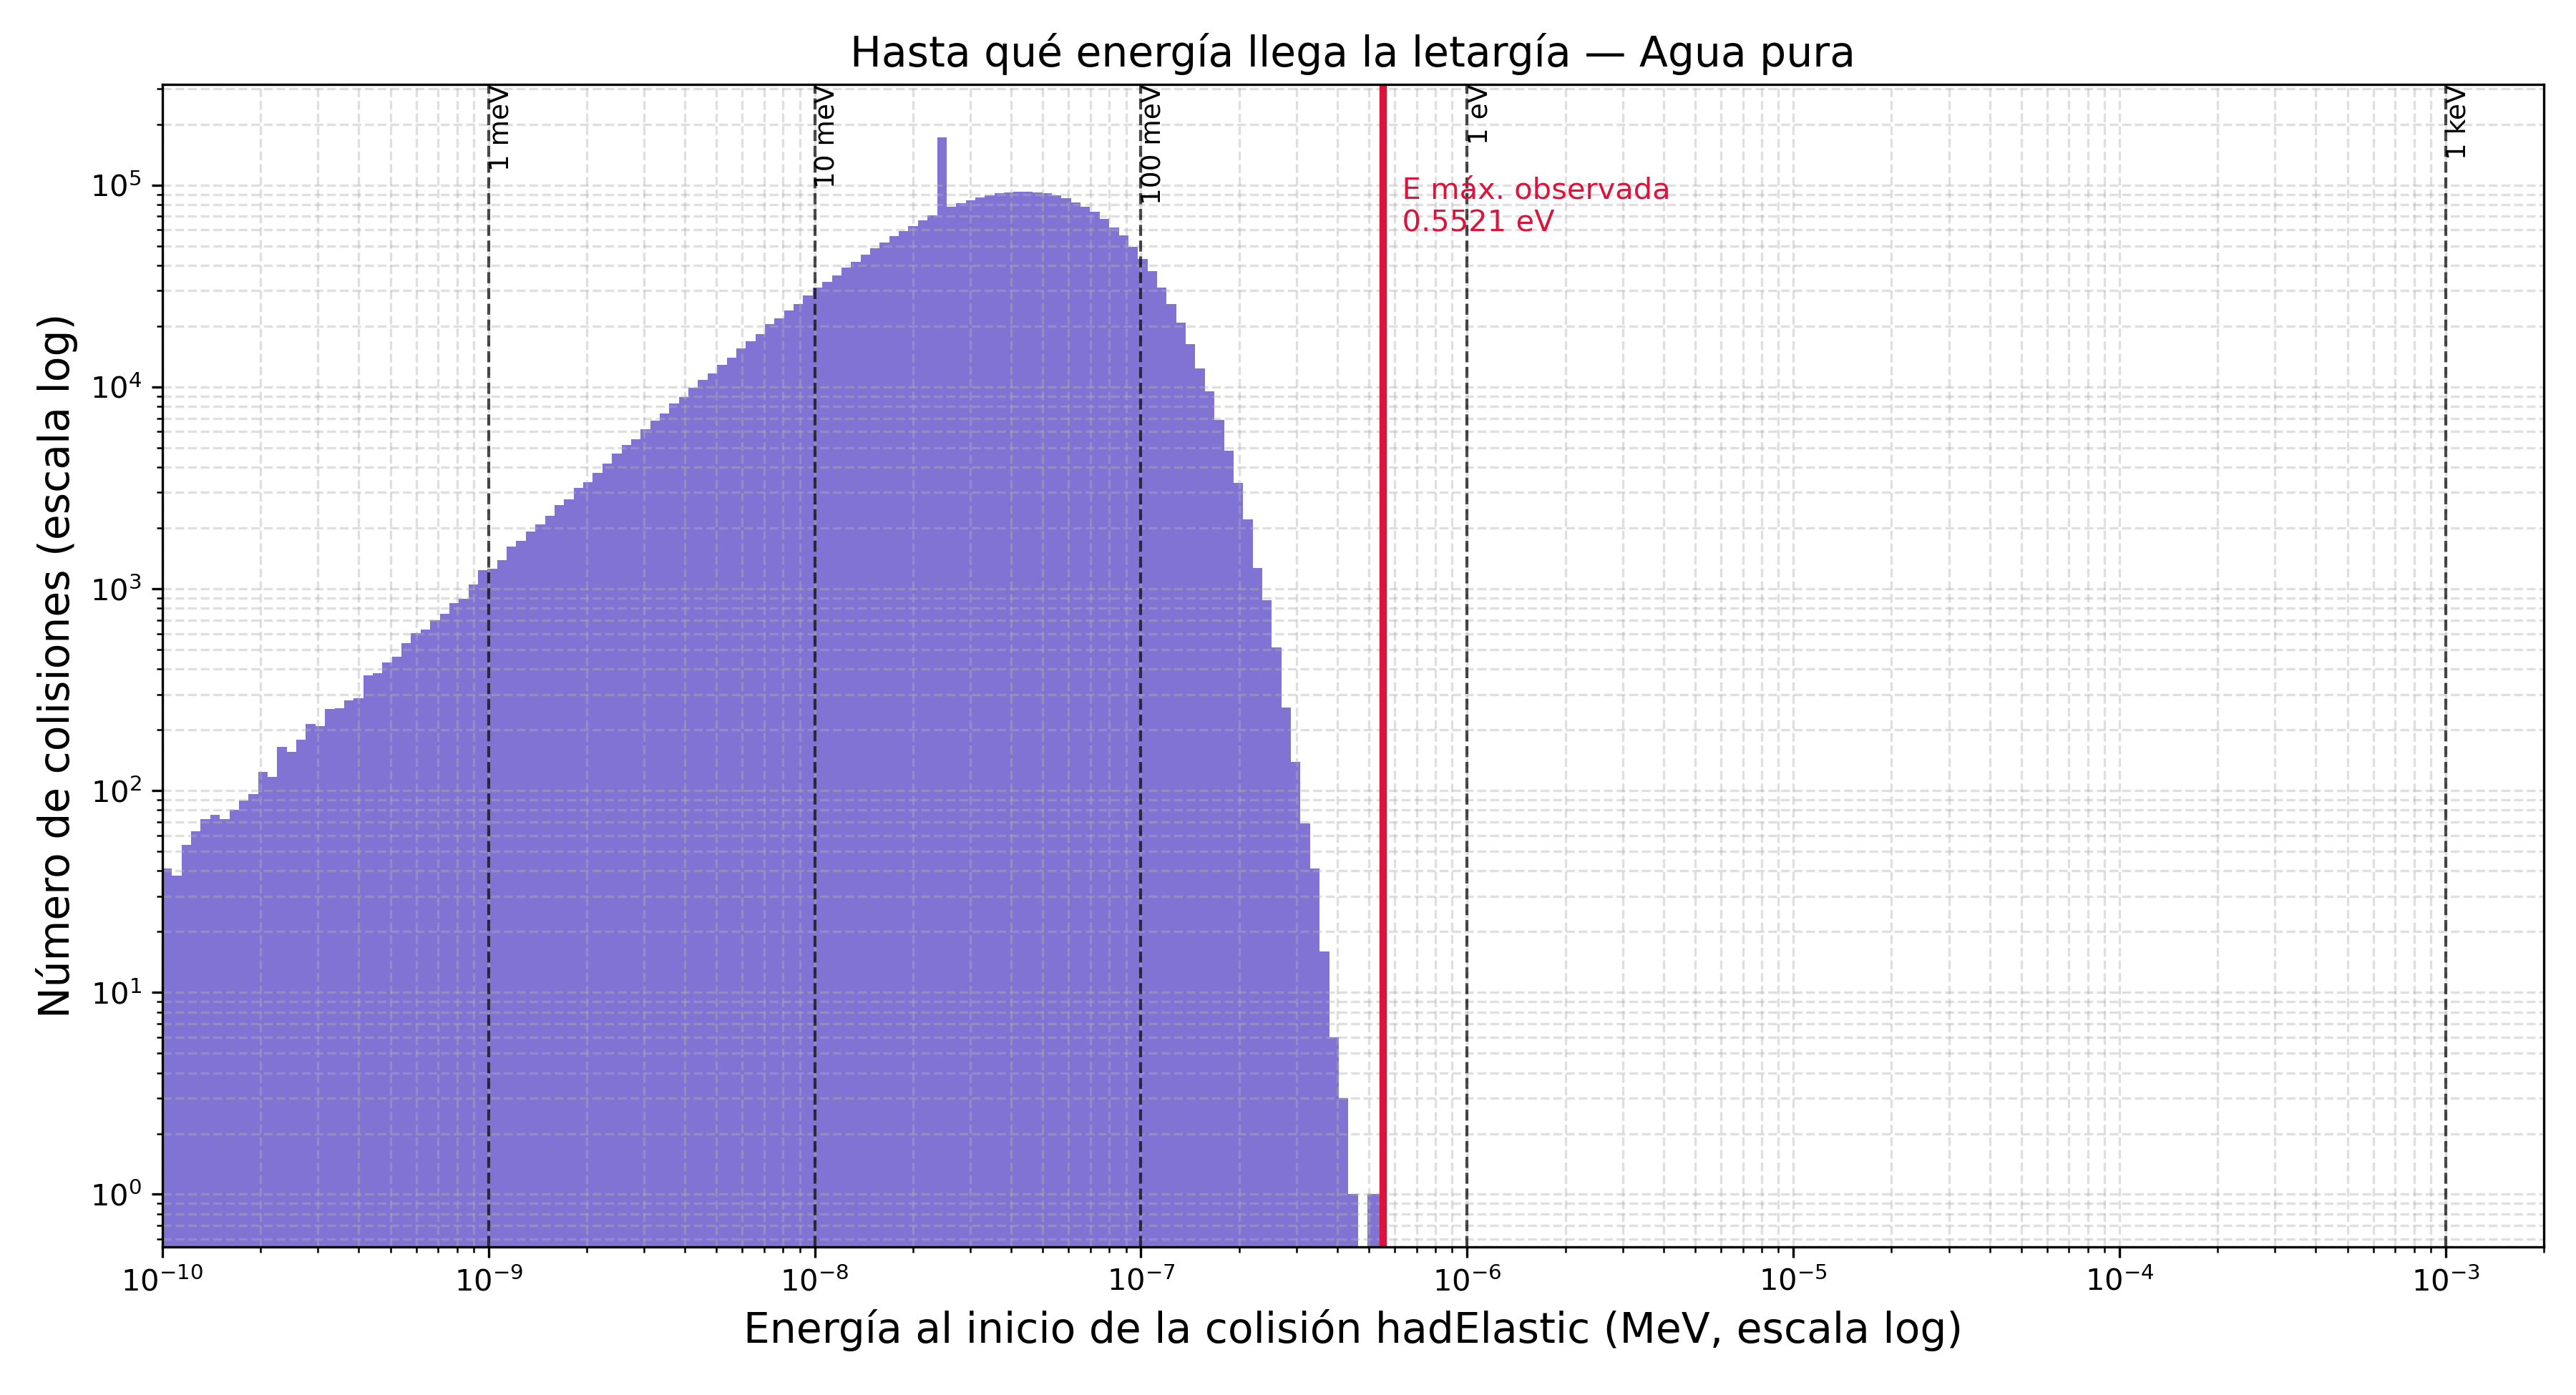
\includegraphics[width=\linewidth]{figuras-analisis-energia/hasta_donde_25meV.png}
    \caption{25\,meV: el régimen Intermedio (entre las líneas de 1\,eV y 1\,keV) queda vacío.}
  \end{subfigure}
  \hfill
  \begin{subfigure}[b]{0.49\linewidth}
    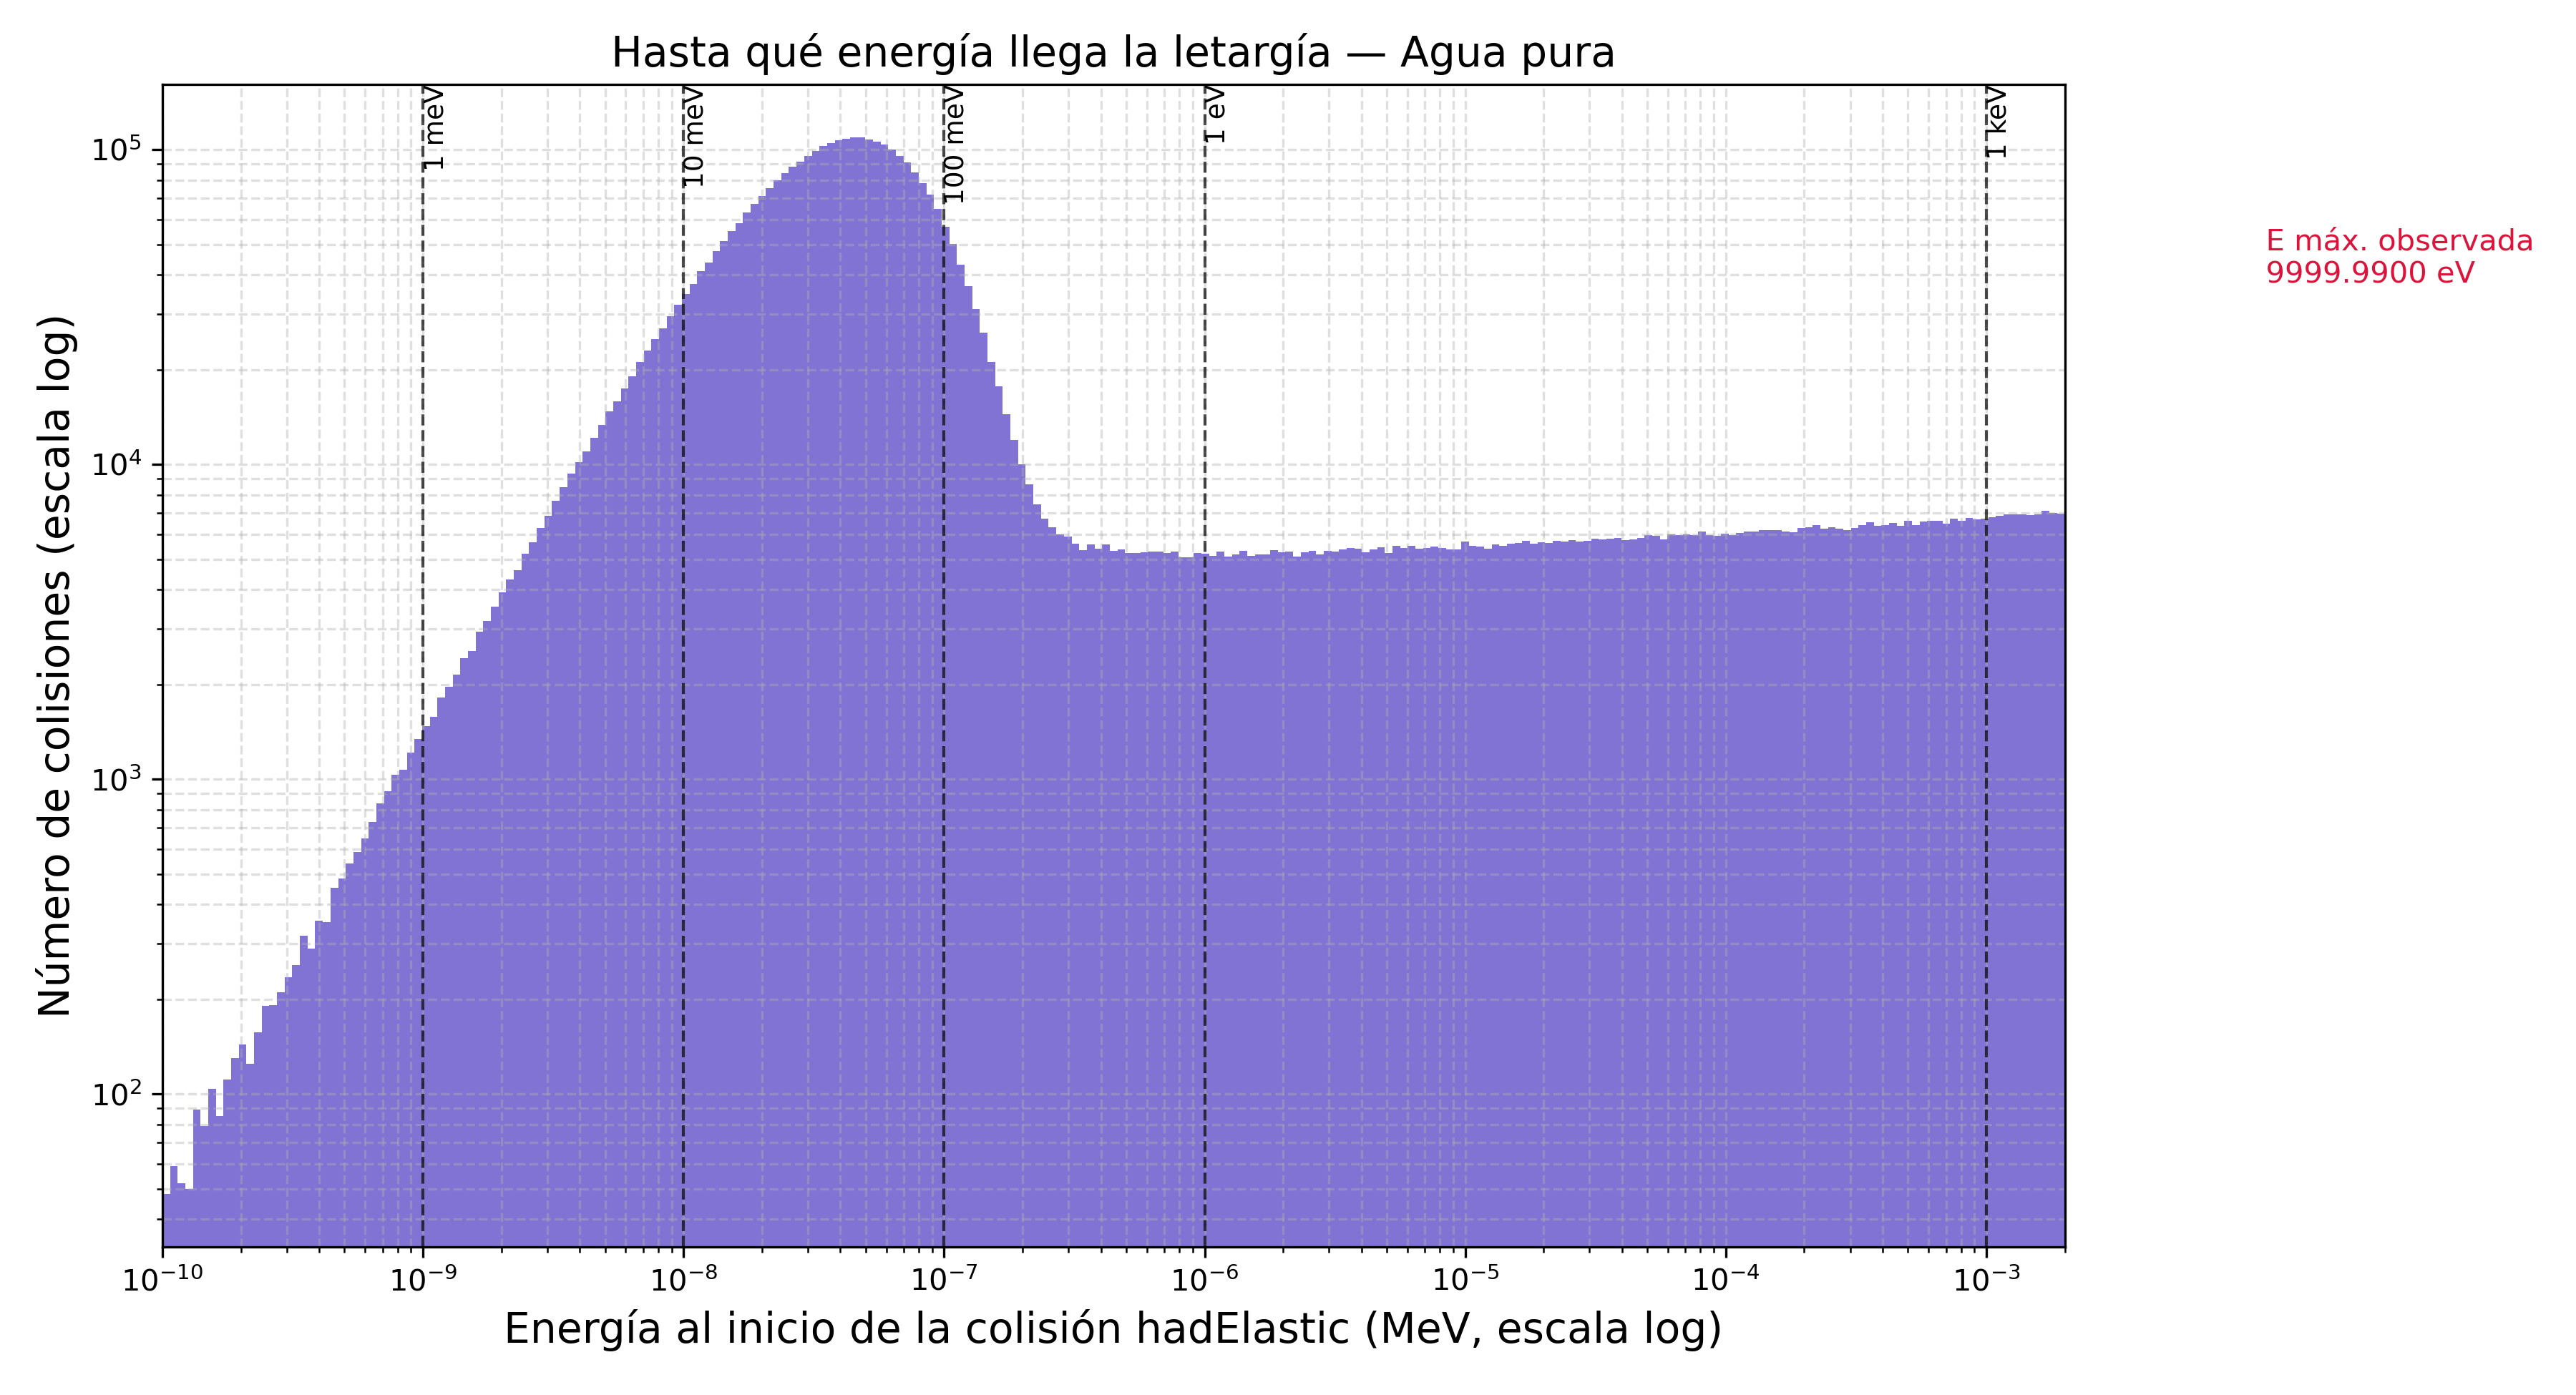
\includegraphics[width=\linewidth]{figuras-analisis-energia/hasta_donde_10keV.png}
    \caption{10\,keV: la fuente parte por encima de 1\,keV y desciende atravesando el régimen
    Intermedio.}
  \end{subfigure}
  \caption{Histograma (escala log-log) de la energía de cada colisión \var{hadElastic}, agua pura,
  con los límites de régimen marcados. La energía máxima observada (línea roja) determina si el
  régimen Intermedio tiene población.}
  \label{fig:hasta_donde}
\end{figure}

\subsection{Número de dispersiones elásticas antes de la captura, $N$}
\label{sec:N}

$N$ es, por neutrón capturado (cualquier material, sección~\ref{sec:limitacion}), el número total de
colisiones \var{hadElastic} en toda su historia. La figura~\ref{fig:N} compara su distribución
$P(N\mid\text{captura})$ entre los cuatro medios, a 25\,meV y a 10\,keV.

\begin{figure}[H]
  \centering
  \begin{subfigure}[b]{0.49\linewidth}
    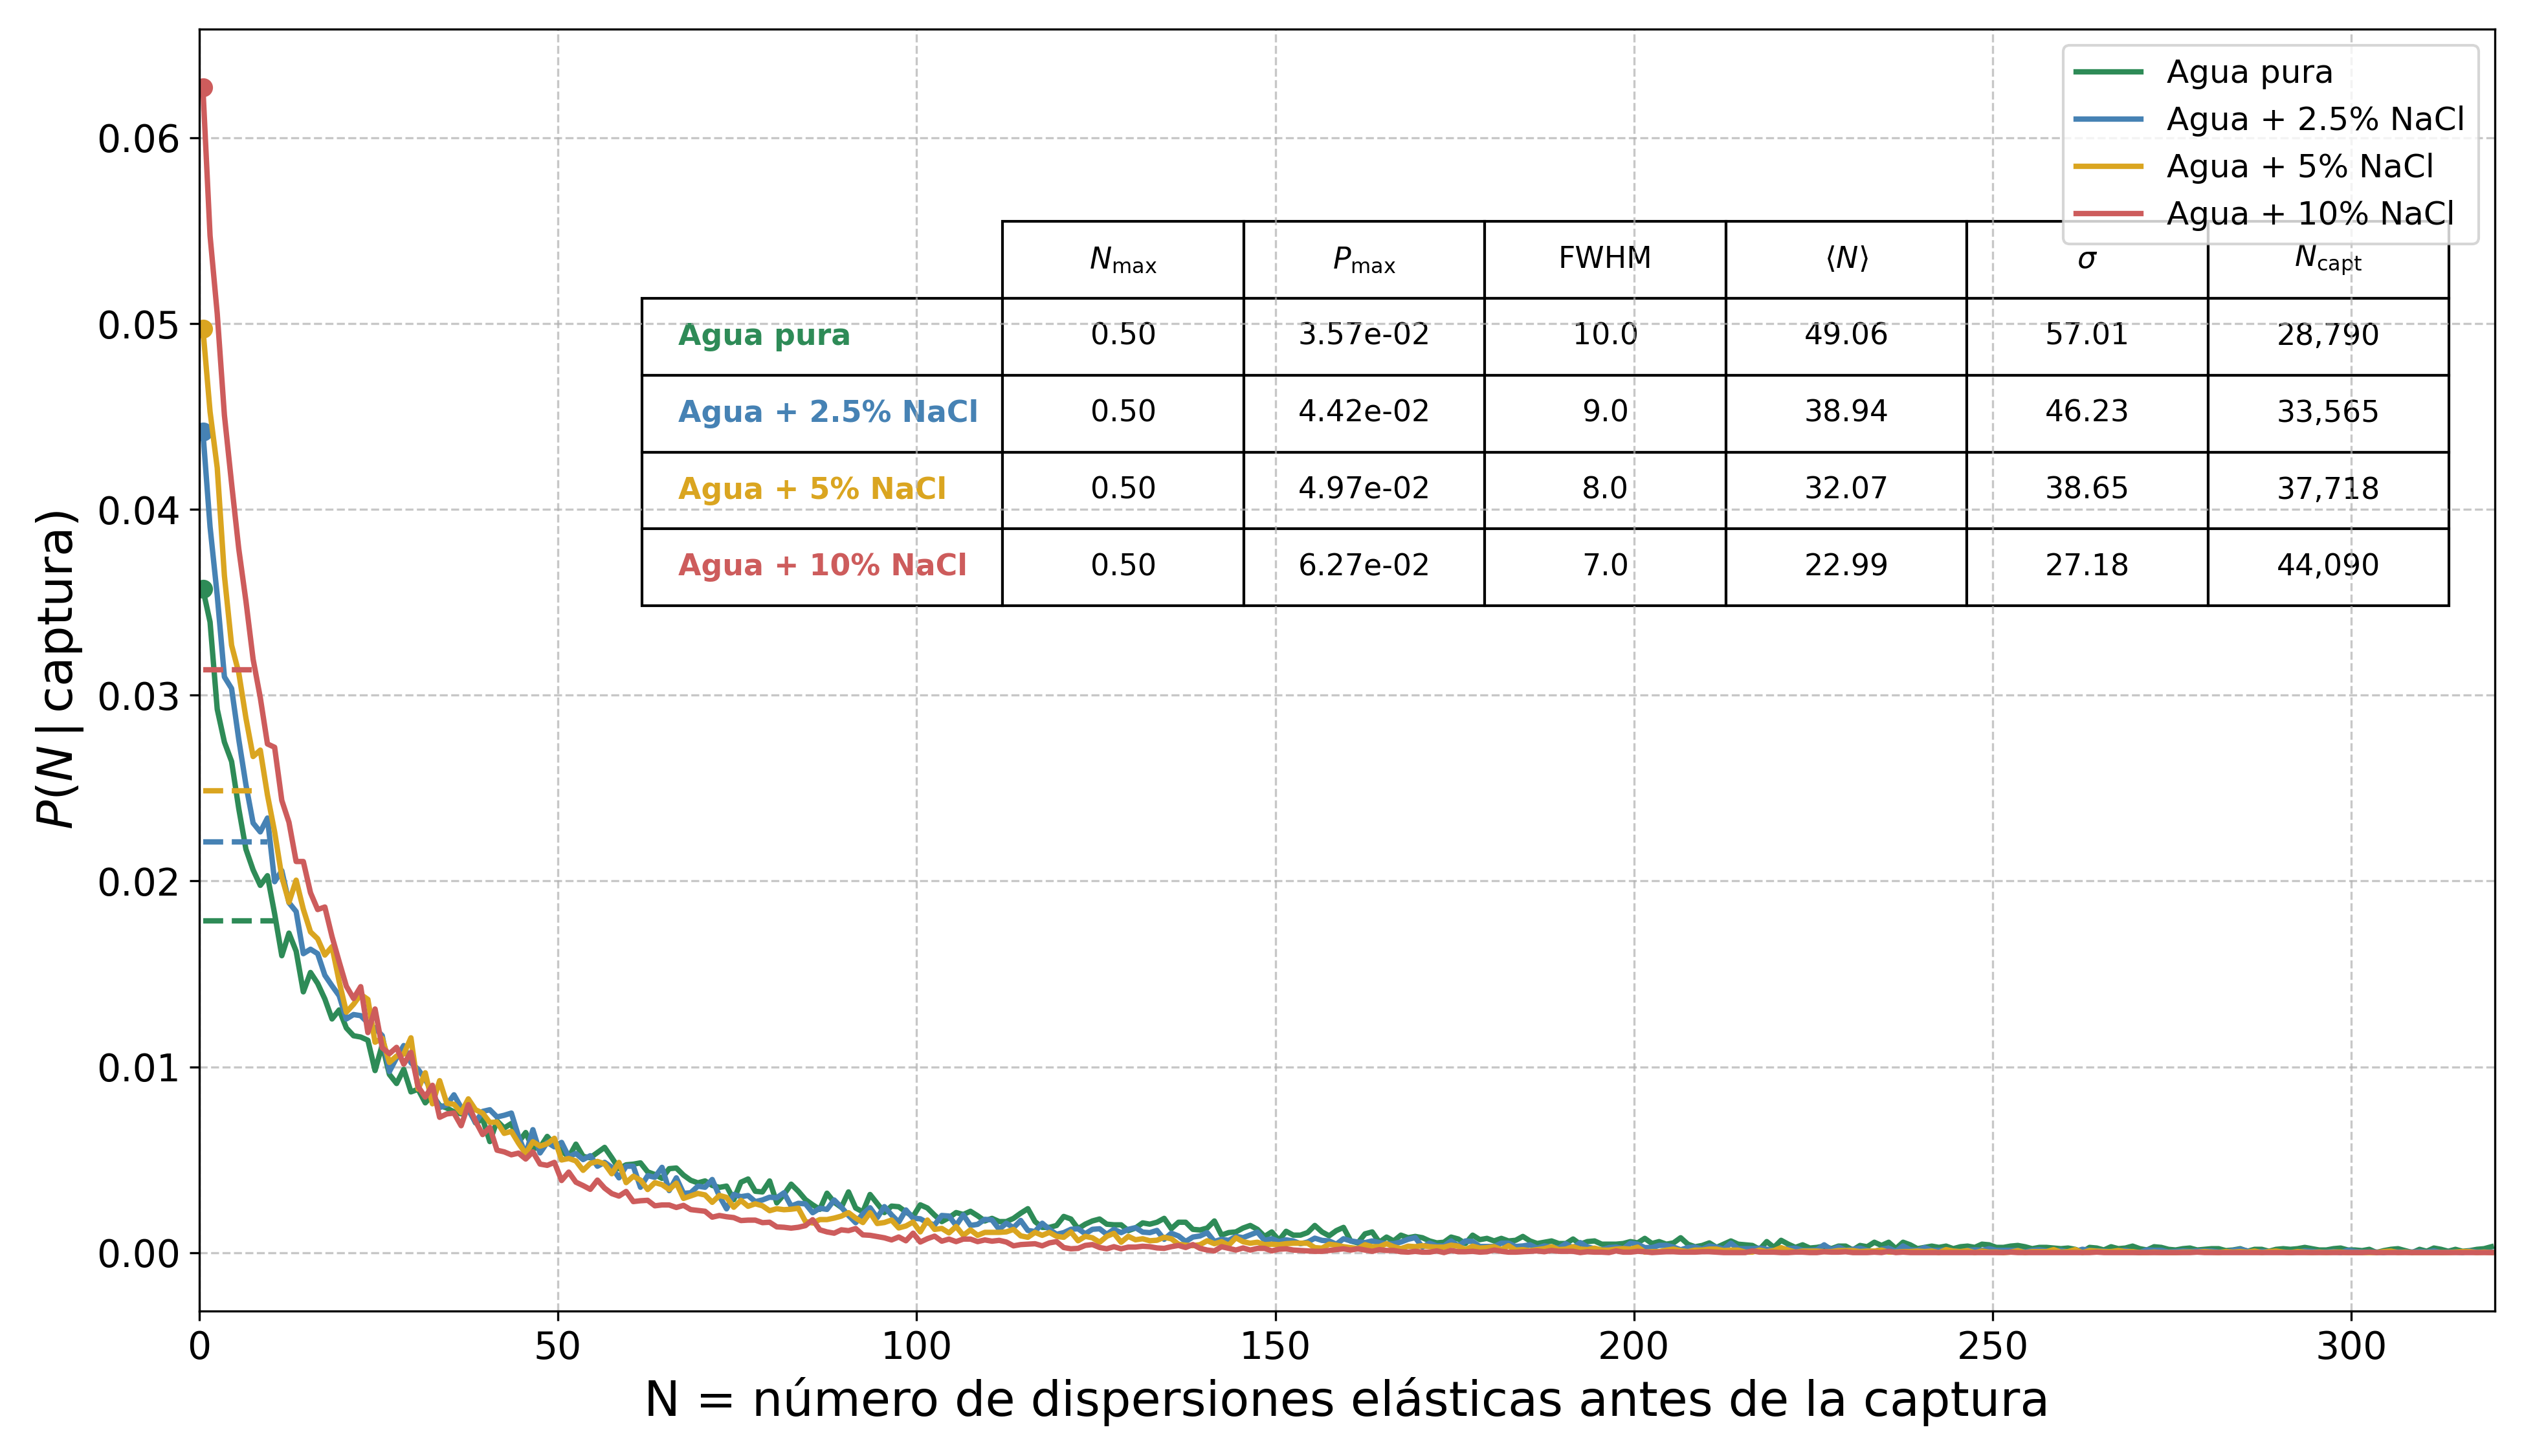
\includegraphics[width=\linewidth]{figuras-analisis-energia/N_25meV.png}
    \caption{25\,meV}
  \end{subfigure}
  \hfill
  \begin{subfigure}[b]{0.49\linewidth}
    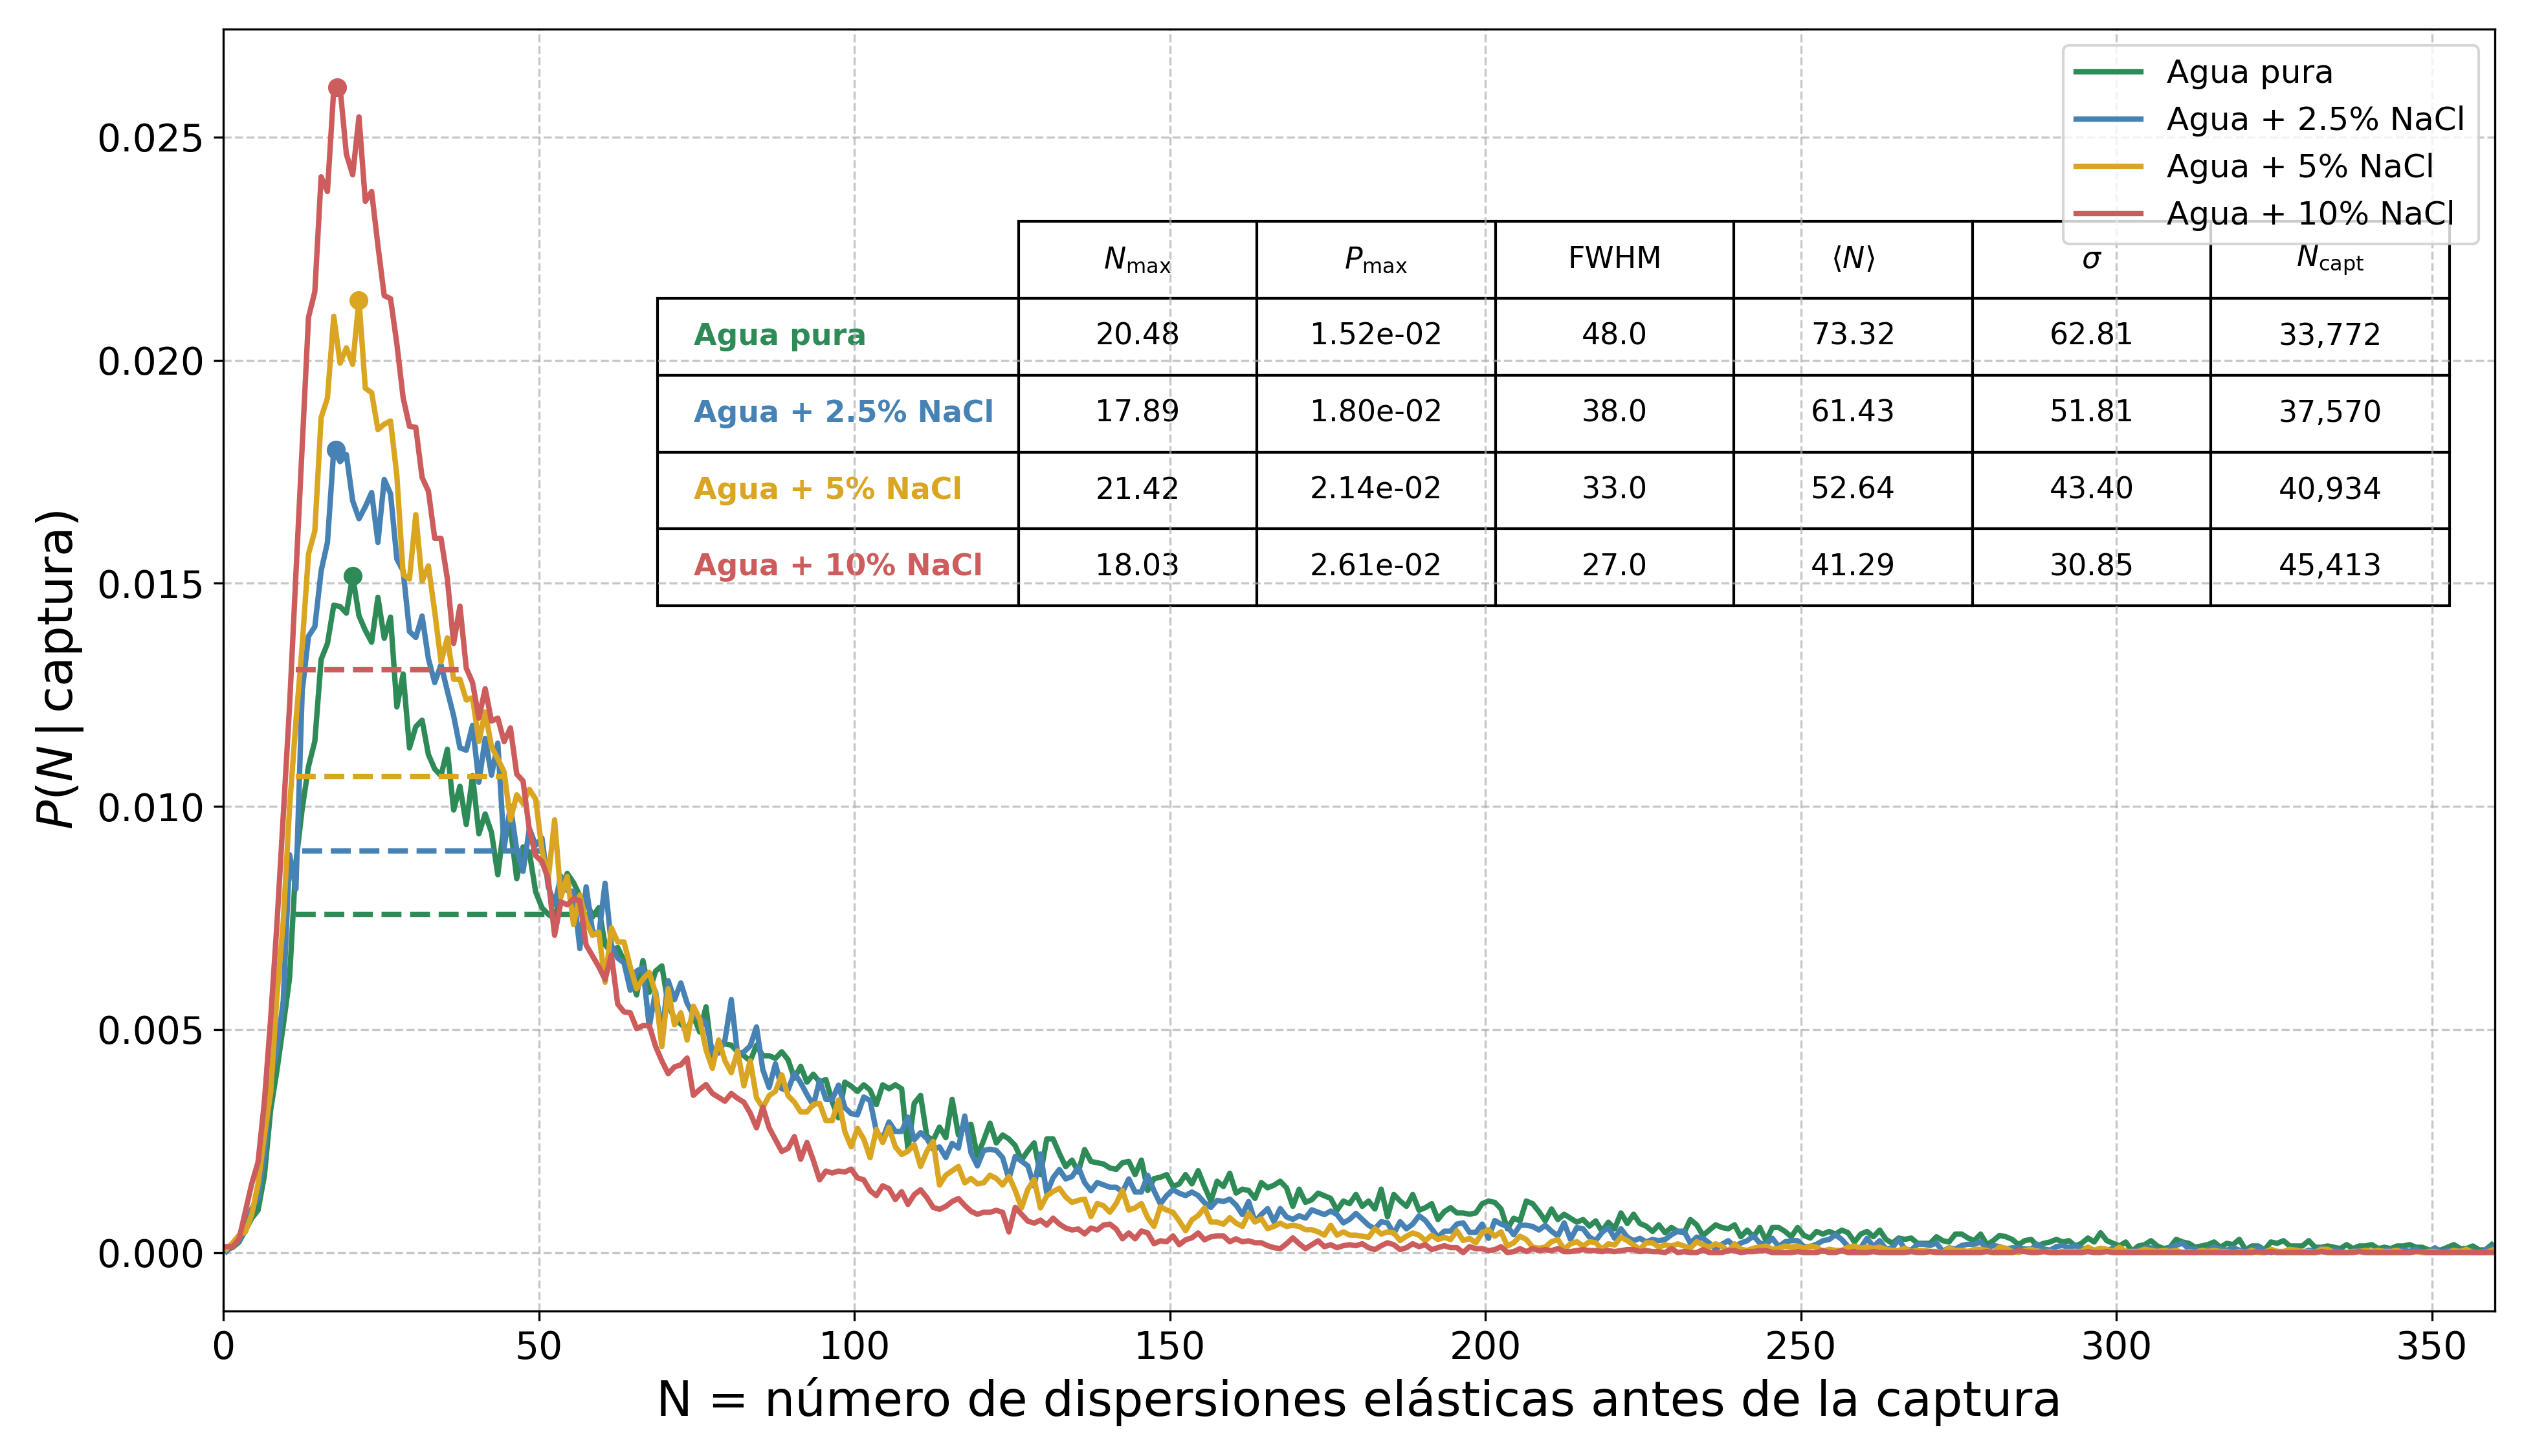
\includegraphics[width=\linewidth]{figuras-analisis-energia/N_10keV.png}
    \caption{10\,keV}
  \end{subfigure}
  \caption{Distribución normalizada de $N$ por medio. En ambas energías, más NaCl desplaza la curva
  hacia $N$ más bajo (captura más rápida); a 10\,keV el valor absoluto de $N$ es más alto porque
  hacen falta colisiones adicionales solo para moderar desde keV hasta el rango térmico.}
  \label{fig:N}
\end{figure}

\subsection{Letargía logarítmica de la historia completa, $\xi$}
\label{sec:xi}

Además de la letargía por régimen (sección~\ref{sec:regimen}), se calcula
$\xi=\ln(E_{\text{pre}}/E_{\text{post}})$ evaluada en \emph{todas} las colisiones \var{hadElastic} de
la historia completa de cada neutrón capturado (sin restringir al volumen detector), y se promedia:
$\langle\xi\rangle$ es la letargía media de esa historia. Esta es la variable donde aparece el
resultado más importante de este informe. La figura~\ref{fig:xi} compara su distribución entre los
cuatro medios, a 25\,meV y a 10\,keV.

\begin{figure}[H]
  \centering
  \begin{subfigure}[b]{0.49\linewidth}
    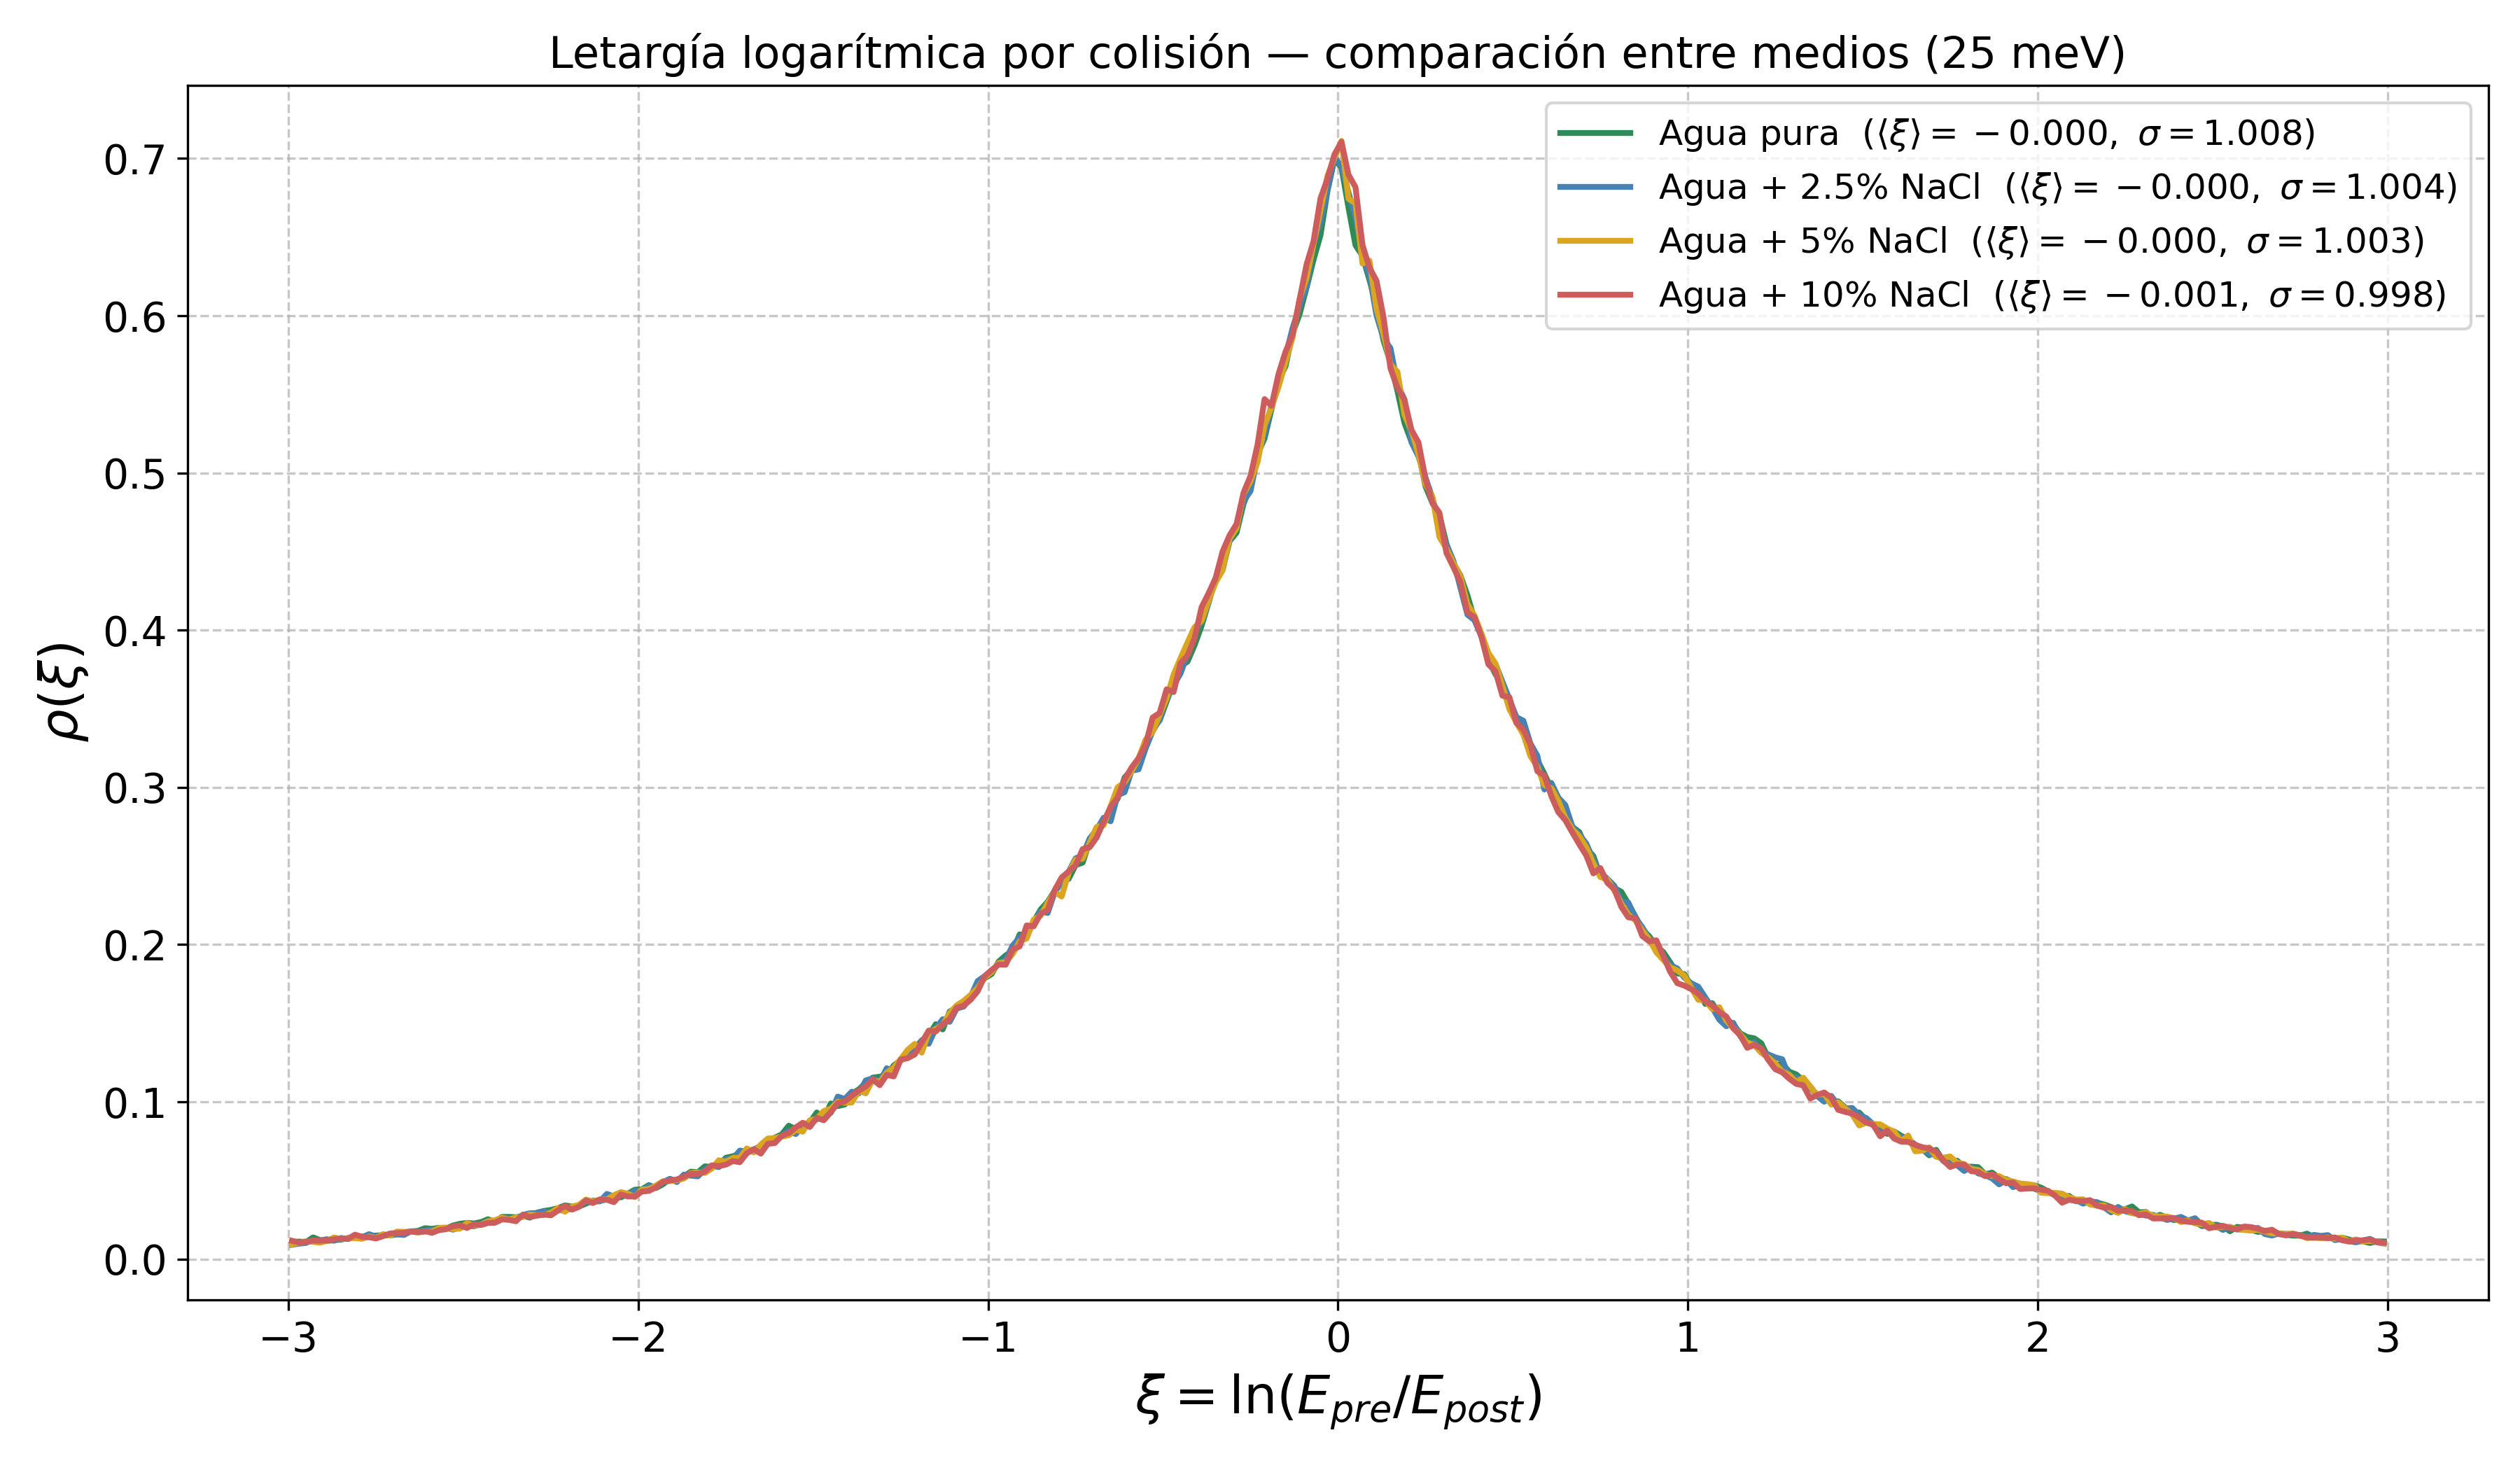
\includegraphics[width=\linewidth]{figuras-analisis-energia/xi_25meV.png}
    \caption{25\,meV: $\langle\xi\rangle\approx 0$, curvas casi indistinguibles entre medios.}
  \end{subfigure}
  \hfill
  \begin{subfigure}[b]{0.49\linewidth}
    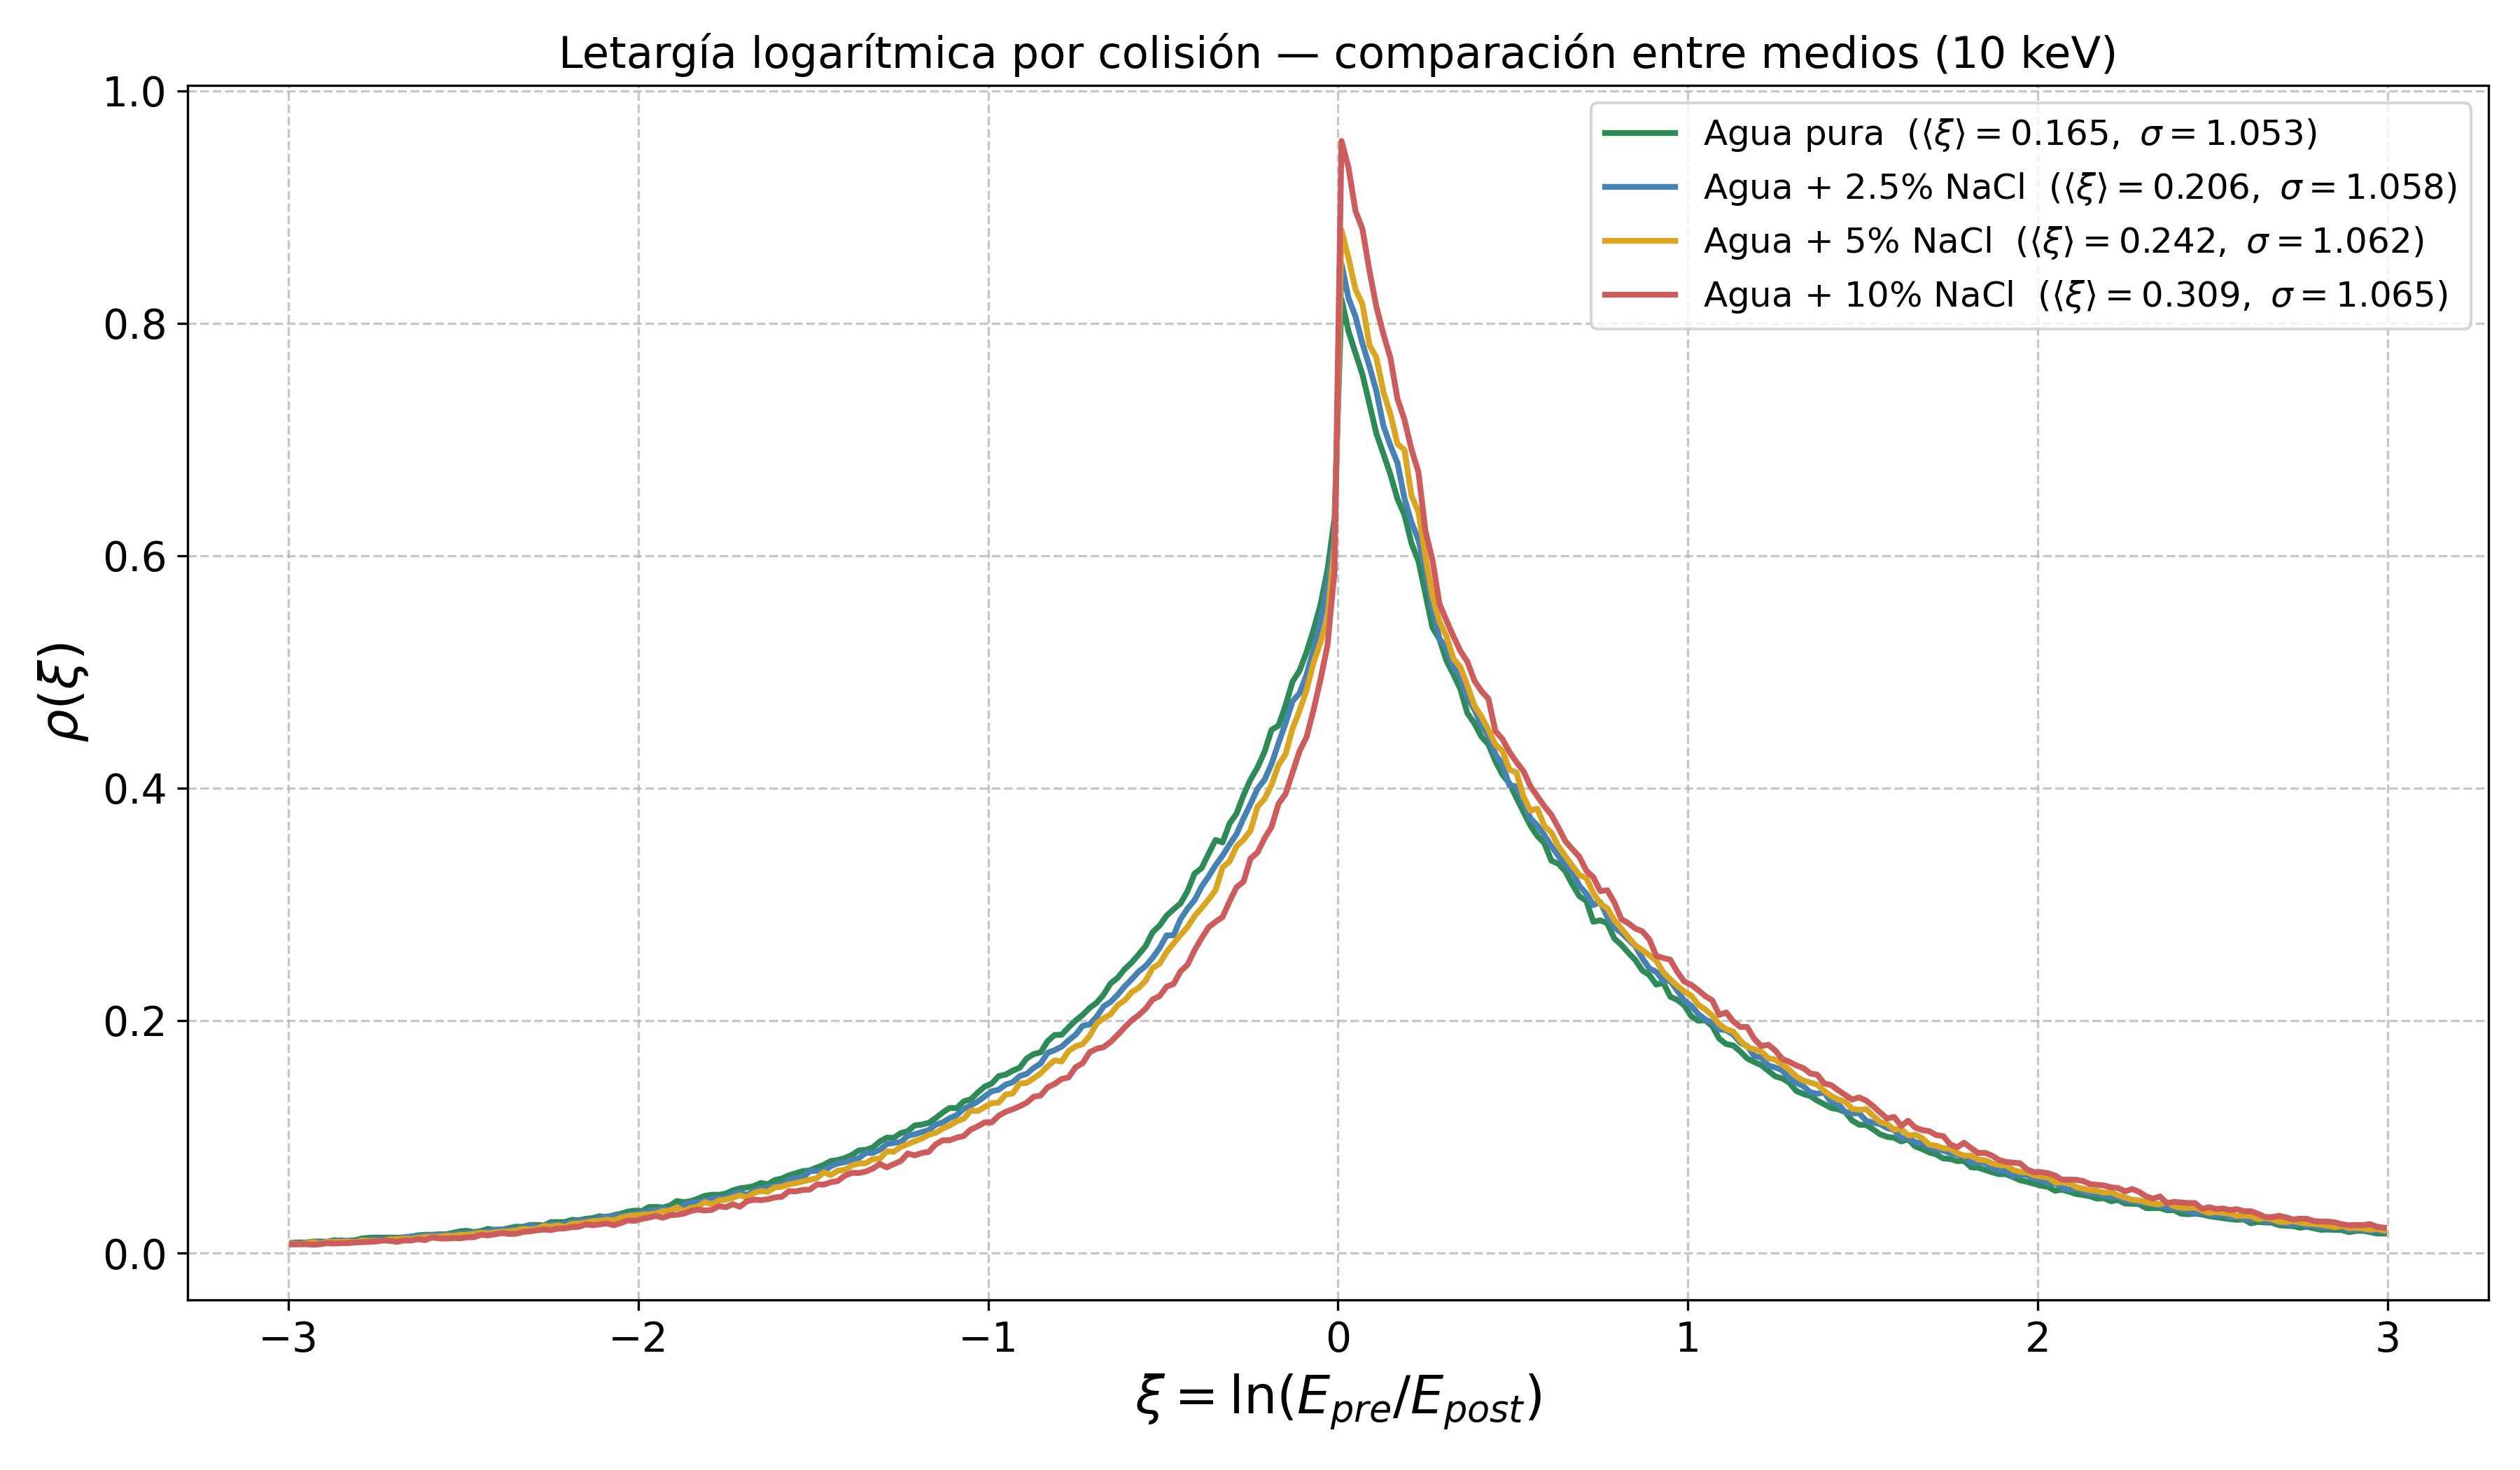
\includegraphics[width=\linewidth]{figuras-analisis-energia/xi_10keV.png}
    \caption{10\,keV: $\langle\xi\rangle$ fuertemente positivo, y las curvas se separan claramente
    con el NaCl.}
  \end{subfigure}
  \caption{Densidad de probabilidad de $\xi$ (historia completa de neutrones capturados), por medio.
  A 25\,meV la fuente ya está termalizada y $\xi$ apenas depende del medio; a 10\,keV domina el
  descenso de moderación (down-scattering) y el NaCl, al acelerar la captura, hace que la historia
  capturada quede más pesada hacia esa fase inicial.}
  \label{fig:xi}
\end{figure}

\section{Resultados comparativos entre las cinco energías}
\label{sec:resultados}

La figura~\ref{fig:tendencias} y la tabla~\ref{tab:comparativa} resumen, para las cinco energías y
los cuatro medios (20 corridas en total), $\langle\xi\rangle$, $\langle N\rangle$ y el porcentaje
capturado.

\begin{figure}[H]
  \centering
  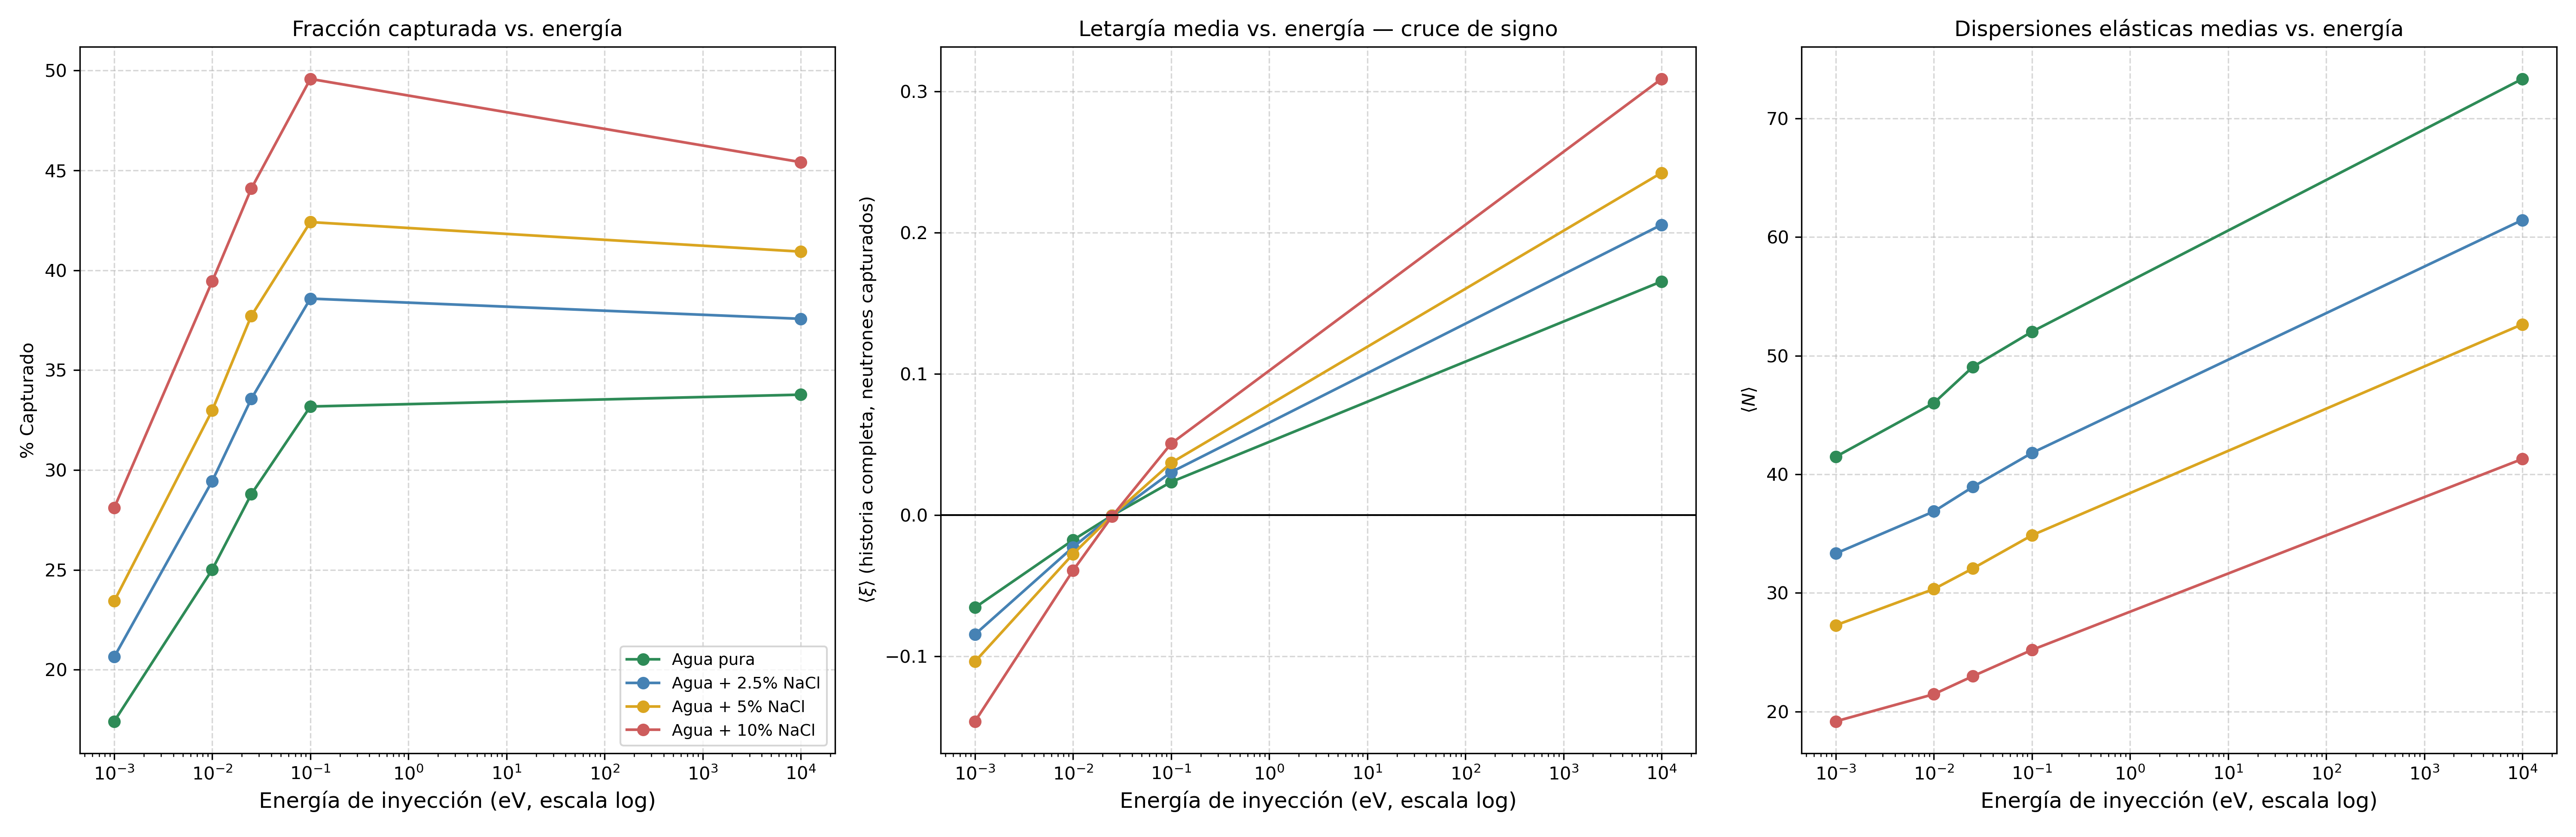
\includegraphics[width=\linewidth]{figuras-analisis-energia/tendencias_vs_energia.png}
  \caption{Porcentaje capturado, $\langle\xi\rangle$ y $\langle N\rangle$ en función de la energía de
  inyección (escala log), una línea por medio. El panel central es el cruce de signo de
  $\langle\xi\rangle$.}
  \label{fig:tendencias}
\end{figure}

\begin{table}[H]
\centering
\small
\begin{tabularx}{\linewidth}{X r r r r r}
\toprule
\textbf{Agua pura} & \textbf{1\,meV} & \textbf{10\,meV} & \textbf{25\,meV} & \textbf{100\,meV} & \textbf{10\,keV} \\
\midrule
\% Capturado & 17.42 & 25.02 & 28.79 & 33.18 & 33.77 \\
\% Reflejado & 55.51 & 53.75 & 51.91 & 49.27 & 49.66 \\
$\langle\xi\rangle$ (historia completa) & $-0.0654$ & $-0.0176$ & $-0.0002$ & $+0.0235$ & $+0.1655$ \\
$\langle N\rangle$ & 41.5 & 46.0 & 49.1 & 52.0 & 73.3 \\
\midrule
\textbf{Agua + 10\,\% NaCl} & & & & & \\
\midrule
\% Capturado & 28.11 & 39.46 & 44.09 & \textbf{49.58} & 45.41 \\
\% Reflejado & 47.62 & 42.65 & 40.40 & 36.68 & 40.72 \\
$\langle\xi\rangle$ (historia completa) & $-0.1459$ & $-0.0391$ & $-0.0007$ & $+0.0507$ & $+0.3088$ \\
$\langle N\rangle$ & 19.2 & 21.5 & 23.0 & 25.2 & 41.3 \\
\bottomrule
\end{tabularx}
\caption{Resumen de las cinco energías, agua pura y agua + 10\,\% NaCl (ver el archivo
\texttt{Salidas/00\_tabla\_maestra\_energias\_medios.tsv} del notebook definitivo, sección
\ref{sec:reprod}, para las 20 filas completas con los cuatro medios).}
\label{tab:comparativa}
\end{table}

Tres observaciones resumen estos resultados:

\begin{itemize}
  \item \textbf{$\langle\xi\rangle$ cambia de signo entre 25\,meV y 100\,meV}, justo alrededor de la
  temperatura ambiente del moderador ($kT\approx25$--$30$\,meV): por debajo domina el
  \textit{up-scattering} inicial mientras el neutrón se termaliza ($\xi<0$); por encima domina el
  descenso normal de moderación ($\xi>0$). La magnitud crece con la distancia al equilibrio en ambas
  direcciones, y en ambas crece también con el NaCl -- porque una captura más rápida (menor $N$) deja
  la historia capturada más pesada hacia la fase inicial de esa historia (fría o caliente, según el
  caso) y menos diluida por las colisiones posteriores cerca del equilibrio.
  \item \textbf{La captura NO es monótona con la energía cuando hay NaCl}: sube de 1\,meV a 100\,meV
  y luego \emph{baja} en 10\,keV (p.\ ej.\ 10\,\% NaCl: 28.1\%$\to$39.5\%$\to$44.1\%$\to$49.6\%
  $\to$45.4\%). En agua pura, en cambio, sigue subiendo (apenas) en el mismo tramo. Una explicación
  plausible, no confirmada con más detalle en este informe: a 10\,keV el neutrón necesita muchas
  colisiones adicionales solo para moderar antes de llegar al rango de energía donde el NaCl ayuda a
  capturarlo, y durante ese descenso largo compite más tiempo contra las categorías de escape.
  \item \textbf{$\langle N\rangle$ sí es monótono con la energía en los cuatro medios}, sin excepción,
  aunque por dos mecanismos distintos: el aumento suave de 1 a 100\,meV refleja que una fuente muy
  fría se captura un poco más rápido (mayor sección eficaz 1/v) antes de acabar de difundirse; el
  salto grande hacia 10\,keV refleja las colisiones adicionales necesarias para moderar desde keV
  hasta el rango térmico.
\end{itemize}

\section{Relación con la aplicación final del WCD}

Un WCD desplegado en campo para CRNS recibe un espectro de neutrones, no un haz monoenergético; ese
espectro depende de cuánto se moderaron los neutrones cósmicos en el suelo (relacionado con la
humedad) y en el aire antes de llegar al detector. Los resultados de este informe muestran que la
respuesta del propio detector --qué fracción se captura, y con qué letargía media-- \textbf{depende
fuertemente de dónde esté ese espectro respecto al equilibrio térmico del agua}: un WCD que reciba
neutrones ya termalizados (como en la mayoría de los estudios de esta tesis, a 25\,meV) tiene una
respuesta distinta --y una dependencia distinta de la concentración de NaCl-- que uno que reciba una
fracción apreciable de neutrones epitérmicos o más rápidos. Esto es relevante al momento de calibrar
un WCD de campo real: la curva de captura \textit{vs.} concentración de NaCl que se use para inferir
salinidad no es universal, sino que depende de la forma del espectro incidente, y este informe
cuantifica exactamente cómo.

\section{Reproducibilidad}
\label{sec:reprod}

Cada corrida se analiza con un notebook individual, con nombre de la forma
\begin{center}
\texttt{Analisis-Balance-Captura-Reflexion-Transmision-<medio>-<energía>.ipynb}
\end{center}
que vive junto a
\archivo{interaccion-completa-neutrones.txt} (o lo genera desde
\archivo{informacion-completa.txt} si no existe) y produce, en su propia carpeta
\archivo{Salidas/}, las tablas y figuras citadas en este informe (incluida la tabla por régimen de
energía y la nota física sobre el régimen Intermedio). Por cada energía, un notebook comparativo
\codigo{Comparacion-4-Medios-<energía>.ipynb} superpone los cuatro medios reutilizando esas tablas ya
calculadas (sin reprocesar los archivos crudos). Finalmente,
\codigo{Resumen-Definitivo-Comparacion-Energias.ipynb} (en la raíz del árbol de simulaciones) junta
las cinco energías reutilizando, a su vez, los \texttt{.tsv} ya generados por los notebooks
anteriores -- es la fuente de la figura~\ref{fig:tendencias}, la tabla~\ref{tab:comparativa} completa
(\archivo{Salidas/00_tabla_maestra_energias_medios.tsv}) y este informe.

Estos notebooks de la Campaña 1 (sección~\ref{sec:campanas}) viven junto a los datos crudos, fuera de
este repositorio (los \texttt{.txt}/\texttt{.tsv} de cada corrida ocupan cientos de MB a varios GB), y
no están replicados en \archivo{analysis/notebooks/} del repositorio; esa carpeta contiene, por ahora,
solo los notebooks de la Campaña 2 (con $S(\alpha,\beta)$).

\section{Conclusiones}

Este informe caracterizó el balance de captura/reflexión/transmisión y la letargía de neutrones en
el WCD a lo largo de cinco energías de inyección (1\,meV a 10\,keV) y cuatro concentraciones de
NaCl, a partir de un pipeline sin información de material (limitación explicada en la
sección~\ref{sec:limitacion}, que impide comparar directamente sus cifras de captura con el
$\eta_{\text{Cap}}$ del resto de la tesis). Los hallazgos centrales son: (1) $\langle\xi\rangle$
--la letargía media de la historia completa de un neutrón capturado-- cambia de signo entre 25\,meV
y 100\,meV, justo alrededor del equilibrio térmico del agua, con una magnitud que crece con la
distancia a ese equilibrio y con la concentración de NaCl; (2) el régimen de energía Intermedio
(1\,eV--1\,keV) solo se puebla cuando la fuente inyecta directamente en o por encima de esa banda
(10\,keV en este estudio), nunca por fluctuación térmica desde una fuente más fría; y (3) la fracción
de captura en presencia de NaCl no es monótona con la energía de inyección --tiene un máximo en
100\,meV--, a diferencia del agua pura. Estos resultados indican que la respuesta del WCD frente a la
salinidad no puede caracterizarse con una única energía de referencia: depende de dónde esté el
espectro de neutrones incidente respecto al equilibrio térmico del moderador.

\label{sec:futuro}
Un punto abierto, no resuelto en este informe, es la comparación cuantitativa con la Campaña 2 de
simulación, la que sí incluye el tratamiento térmico $S(\alpha,\beta)$ (sección~\ref{sec:campanas}):
sus primeros resultados, disponibles hasta ahora a 25\,meV --la misma energía de inyección que la
corrida de agua pura/NaCl de esta campaña a esa energía--, ya muestran una fracción de captura
distinta de la de esta campaña a esa misma energía. Cuantificar sistemáticamente esa diferencia --y
su origen físico en la sección eficaz de dispersión elástica del hidrógeno ligado-- a partir de ese
punto de comparación directa, y extender la Campaña 2 a las otras cuatro energías de este informe,
queda como trabajo futuro.

\end{document}
